\documentclass[a4paper, 9pt]{extarticle}
% (1) Encoding, Fonts, and Layout
\usepackage[T1]{fontenc}
\usepackage{lmodern}
\usepackage[margin=1in]{geometry}


% (2) Common Packages
\usepackage{amsmath, amssymb, amsthm}
\usepackage{xcolor}
\usepackage{caption}
\usepackage{tikz}
\usepackage{pgfplots}
\pgfplotsset{compat=newest}
\usepackage{etoolbox}
\usepackage{tikz-3dplot}
\tdplotsetmaincoords{75}{120}
\usepackage[inline]{enumitem}
\usepackage{bookmark}
\usepackage{mathtools}
\usepackage{subcaption} % For subfigures
\usepackage[normalem]{ulem} % For better underline commands

% Micro-typography
\usepackage{microtype}

% Patching pgfplots warning
\makeatletter
\patchcmd{\pgfplots@applistXXpushback@smallbuf}{\pgfplots@error}{\pgfplots@warning}{}{}
\makeatother

% (3) tcolorbox and Theorem Libraries
\usepackage{tcolorbox}
\tcbuselibrary{theorems}

% (4) Define Colors
\definecolor{custom_green}{HTML}{a3be8c}
\definecolor{custom_red}{HTML}{dc322f}
\definecolor{custom_blue}{HTML}{268bd2}
\definecolor{custom_purple}{HTML}{b48ead}

\definecolor{base}{HTML}{eceff4}
\definecolor{gray1}{HTML}{e5e9f0}
\definecolor{gray2}{HTML}{d8dee9}
\definecolor{gray3}{HTML}{2e3440}
\pagecolor{base}

% (5) Custom tcolorbox Environments
\newtcolorbox{definitionbox}[1][]{
    title=\textbf{Definition} {#1},
    fonttitle=\bfseries\boldmath,
    arc=0mm,
    bottomtitle=0.5mm,
    boxrule=0mm,
    colbacktitle=gray2,
    colback=gray1,
    coltitle=gray3,
    coltext=gray3,
    left=2.5mm,
    leftrule=1mm,
    rightrule=1mm,
    right=3.5mm,
    toptitle=0.75mm,
    colframe=custom_red,
}

\newtcolorbox{proofbox}{
    title=\textbf{Proof},
    fonttitle=\bfseries\boldmath,
    arc=0mm,
    bottomtitle=0.5mm,
    boxrule=0mm,
    colbacktitle=gray2,
    colback=gray1,
    coltitle=gray3,
    left=2.5mm,
    leftrule=1mm,
    rightrule=1mm,
    right=3.5mm,
    toptitle=0.75mm,
    colframe=custom_blue,
    coltext=gray3,
}

\newtcolorbox{theorembox}[1][]{
    title=\textbf{Theorem} {#1},
    fonttitle=\bfseries\boldmath,
    arc=0mm,
    bottomtitle=0.5mm,
    boxrule=0mm,
    colbacktitle=gray2,
    colback=gray1,
    coltitle=gray3,
    left=2.5mm,
    leftrule=1mm,
    rightrule=1mm,
    right=3.5mm,
    toptitle=0.75mm,
    colframe=custom_green,
    coltext=gray3
}

\newtcolorbox{notebox}{
    title=\textbf{Note},
    fonttitle=\bfseries\boldmath,
    arc=0mm,
    bottomtitle=0.5mm,
    boxrule=0mm,
    colbacktitle=gray2,
    coltitle=gray3,
    left=2.5mm,
    leftrule=1mm,
    rightrule=1mm,
    right=3.5mm,
    toptitle=0.75mm,
    colframe=custom_blue,
    coltext=gray3
}

\newtcolorbox{examplebox}[1][]{
    title=\textbf{Example} {#1},
    fonttitle=\bfseries\boldmath,
    arc=0mm,
    bottomtitle=0.5mm,
    boxrule=0mm,
    colbacktitle=gray2,
    colback=gray1,
    coltitle=gray3,
    left=2.5mm,
    leftrule=1mm,
    rightrule=1mm,
    right=3.5mm,
    toptitle=0.75mm,
    colframe=gray3,
    fontupper=\footnotesize,
    coltext=gray3
}

% (6) Theorem Environments
\theoremstyle{definition}
\newtheorem{definition}{Definition}[section]
\newtheorem{example}[definition]{Example}

\theoremstyle{plain}
\newtheorem{theorem}[definition]{Theorem}

% (7) Hyperlinks
\usepackage{hyperref}
\hypersetup{
    colorlinks=true,    % Use colored text for links
    linkcolor=custom_red,      % Set link text color to red
    pdfborder={0 0 0}   % Remove the default box around links
}

% macros.tex
\newcommand{\intinf}{\int_0^{\infty}} % Integral from 0 to infinity
\newcommand{\diff}[2]{\frac{d#1}{d#2}} % Derivative

\usepackage{tikz}
\usetikzlibrary{decorations.pathreplacing}



\usepackage{geometry}
 \geometry{
 a4paper,
 bottom=22mm,
 }

       

\begin{document}
\begin{center}
  Robert Davidson\\
  BSc Mathematics and Computer Science\\[24pt]

  \large
  \textbf{Linear Algebra (MA283) notes}\\[6pt]
  \small
  Date: \today\\[48pt]
  \normalsize
\end{center}
\begin{abstract}
  \begin{adjustwidth}{1cm}{1cm}
    \noindent Linear algebra provides a framework to understand and analyze systems defined by linear equations and transformations, serving as the foundation of diverse areas in mathematics, science, engineering, and beyond. These notes introduce and build upon core concepts, beginning with \textbf{systems of linear equations} and extending into abstract vector spaces, transformations, and geometric interpretations. \\[2ex]
    \noindent We first explore the fundamental notions of \textbf{linear independence}, \textbf{subspaces}, and \textbf{span}, which clarify the structure underlying linear systems. Equipped with these tools, we define \textbf{basis} and \textbf{dimension}, revealing how vector spaces can be succinctly and precisely described. This naturally leads us to \textbf{coordinates}, enabling clear communication about vectors across different bases, and the crucial concepts of \textbf{rank} and \textbf{nullity}, capturing essential properties of linear transformations. \\[2ex]
    \noindent Next, we delve into \textbf{inner products}, \textbf{orthogonality}, and \textbf{projections}, extending geometric intuition into abstract vector spaces. These ideas give rise to practical methods like the Gram-Schmidt process, orthogonal projections, and least squares approximations, which are indispensable in both theoretical and real-world contexts. \\[2ex]
    \noindent Finally, we examine \textbf{eigenvalues}, \textbf{eigenvectors}, and \textbf{diagonalizability}, exploring how linear transformations can be simplified and understood by choosing optimal bases. These powerful tools provide insight into the intrinsic properties of matrices and transformations, enabling deeper analysis and efficient computation. \\[2ex]
    \noindent Together, these notes offer a coherent journey through linear algebra, balancing theoretical depth with practical applications, equipping readers with both the conceptual clarity and computational skills needed to leverage linear algebra across various fields.
  \end{adjustwidth}
\end{abstract}

\pagebreak
\footnotesize
\tableofcontents
\pagebreak
\normalsize
\section{Review of Matrix Algebra}
\subsection*{Matrix Addition}
If a matrix has $m$ rows and $n$ columns, we say it is $m \times n$. \textbf{Two matrices can only be added if they have the same size.}. In this case, we just add the entries in each position. \\[1.5ex]
The $m \times n$ \textbf{zero} matrix is a matrix with all entries equal to $0$. It is the \textbf{Identity element} for matrix addition (adding it to any matrix does not change the matrix)
\subsection*{Matrix Multiplication by a Scalar}
This simply means multiplying each entry of the matrix by the scalar. For example:
$$
  \alpha \begin{bmatrix}
    1 & 2 \\
    3 & 4 \\
  \end{bmatrix}
  =
  \begin{bmatrix}
    \alpha  & 2\alpha \\
    3\alpha & 4\alpha \\
  \end{bmatrix}
$$
\subsection*{Vector Space}
\begin{definitionbox}{}{}
  The most typical example of a \textbf{vector space} is $\mathbb{R}^n$, the all $n$ sized vector of real numbers
  $$\{(x_1, \dots, x_n)\; x_i \in \mathbb{R}\}$$
  What makes this a vector space is is that we can add two $n$-vector together:
  $$(x_, \dots, x_n) + (y_1, \dots, y_n) = (x_1 + y_1, dots, x_n + y_n)$$
  and we can multiply each vector by a scalar, $\alpha$:
  $$
    \alpha (x_1, \dots, x_n) = (\alpha x_1, \dots, \alpha x_n)
  $$
\end{definitionbox}

\subsection*{Linear Combinations}
Suppose $v_1, v_2, \dots, v_k$ are elements that can be added together and multiplied by scalars. \\[2ex]
A Linear Combination of $v_1, v_2, \dots, v_k$ is an expression of the form:
$$
  \alpha_1 v_1 + \alpha_2 v_2 + \ldots + \alpha_k v_k
$$
where $a_i \in \mathbb{R}$ are scalars, called \textbf{coefficients}.
\subsection*{Matrix-Vector Multiplication}
Let $A$ be a $m \times n$ matrix, and $\textbf{v}$ be a column vector with $n$ entries ($n \times 1$ matrix). \\[2ex]
Then the matrix vector product $Av$ is the column vector, with $m$ entries, obtained by taking the linear combination of the columns of $A$ with the entries of $\textbf{v}$ as coefficients. \\
\textbf{Example:}
$$
  \begin{bmatrix}
    -1 & 2 & 4 \\
    0  & 1 & 3
  \end{bmatrix}
  \begin{bmatrix}
    7 \\
    6 \\
    9
  \end{bmatrix}
  =
  7 \begin{bmatrix}
    -1 \\
    0
  \end{bmatrix}
  + 6 \begin{bmatrix}
    2 \\
    1
  \end{bmatrix}
  + 9 \begin{bmatrix}
    4 \\
    3
  \end{bmatrix}
  =
  \begin{bmatrix}
    41 \\
    33
  \end{bmatrix}.
$$
\textbf{Remark:} $Av$, if defined, has the same number of rows as $A$ and the same number of columns as $\textbf{v}$.

\subsection*{Matrix-Matrix Multiplication}

Let $A$ and $B$ be matrices of size $m \times $ and $p \times n$, respectively.Write $v_1, \ldots v_n$ for the columns of $B$. Then the product $AB$ is the $m \times n$ matrices whose columns are $Av_1 , \ldots, Av_n$. \\[2ex]
The entry at row $i$ and column $j$ of the matrix $A$ is given by $A_{ij}$. The entry in the $i,j$ position of the product $AB$ is the $i$th entry of the vector $Av_j$, where the vector $v_j$ is the $j$th column of $B$. In other words, the entry in the $i,j$ position of the product $AB$ is given by:
$$
  (AB)_{ij} = A_{i1}B_{1j} + A_{i2}B_{2j} + \ldots + A_{ip}B_{pj} = \sum_{k=1}^p A_{ik}B_{kj}
$$
Alternatively, if $A$ is $m \times p$ with rows $u_1, \ldots, u_m$ and $B$ is $p \times n$ with columns $v_1, \ldots, v_n$, then the product $AB$ is:
$$AB =
  \begin{bmatrix}
    u_1 \cdot v_1 & u_1 \cdot v_2 & \ldots & u_1 \cdot v_n \\
    u_2 \cdot v_1 & u_2 \cdot v_2 & \ldots & u_2 \cdot v_n \\
    \vdots        & \vdots        & \ddots & \vdots        \\
    u_m \cdot v_1 & u_m \cdot v_2 & \ldots & u_m \cdot v_n
  \end{bmatrix}
$$
\textbf{Example}:
$$
  A =
  \begin{bmatrix}
    1 & 2 & 3 \\
    4 & 5 & 6
  \end{bmatrix}
  \quad
  B =
  \begin{bmatrix}
    7  & 8  \\
    9  & 10 \\
    11 & 12
  \end{bmatrix}
  \quad
  AB =
  \begin{bmatrix}
    1 \cdot 7 + 2 \cdot 9 + 3 \cdot 11 & 1 \cdot 8 + 2 \cdot 10 + 3 \cdot 12 \\
    4 \cdot 7 + 5 \cdot 9 + 6 \cdot 11 & 4 \cdot 8 + 5 \cdot 10 + 6 \cdot 12
  \end{bmatrix}
  =
  \begin{bmatrix}
    58  & 64  \\
    139 & 154
  \end{bmatrix}
$$
For matrices $A$ and $B$, the products $AB$ and $BA$ are generally not
equal, even if they are both defined and even if both have the same
size.
\subsection*{Linear Transformations}

Let $m$ and $n$ be positive integers. \\[2ex]
A \textbf{linear transformation} $T$ from $\mathbb{R}^n$ to $\mathbb{R}^m$ is a function $T:\mathbb{R}^n \to \mathbb{R}^m$ that satisfies:
\begin{itemize}
  \item $T(\textbf{u} + \textbf{v}) = T(\textbf{u}) + T(\textbf{v})$ for all $\textbf{u}, \textbf{v} \in \mathbb{R}^n$
  \item $T(\lambda\textbf{u}) = \lambda T(\textbf{u})$ for all $\textbf{u} \in \mathbb{R}^n$ and $\lambda \in \mathbb{R}$
\end{itemize}

\subsection*{Matrix of a Linear Transformation}
Suppose $T:\mathbb{R}^3 \to \mathbb{R}^2$ is the linear transformation:
$$
  T\begin{bmatrix}
    1 \\
    0 \\
    0 \\
  \end{bmatrix}
  = \begin{bmatrix}
    2 \\
    3 \\
  \end{bmatrix}
  \quad
  T\begin{bmatrix}
    0 \\
    1 \\
    0 \\
  \end{bmatrix}
  = \begin{bmatrix}
    1 \\
    4 \\
  \end{bmatrix}
  \quad
  T\begin{bmatrix}
    0 \\
    0 \\
    1 \\
  \end{bmatrix}
  = \begin{bmatrix}
    -6 \\
    7  \\
  \end{bmatrix}
$$
Then for the vector in $\mathbb{R}^3$ with entries $a,b,c$:
$$
  T\begin{bmatrix}
    a \\
    b \\
    c \\
  \end{bmatrix}
  = aT\begin{bmatrix}
    1 \\
    0 \\
    0 \\
  \end{bmatrix}
  + bT\begin{bmatrix}
    0 \\
    1 \\
    0 \\
  \end{bmatrix}
  + cT\begin{bmatrix}
    0 \\
    0 \\
    1 \\
  \end{bmatrix}
  = \begin{bmatrix}
    2  & 1 & -6 \\
    -3 & 4 & 7
  \end{bmatrix}
  \begin{bmatrix}
    a \\
    b \\
    c
  \end{bmatrix}
$$
Where the $2\times 3$ matrix $M_T$ is called the \textbf{standard matrix} of A.
A linear transformation $T: \mathbb{R}^n \rightarrow \mathbb{R}^m$ can be completely represented by an $m \times n$ matrix $M_T$. \\[2ex]
\textbf{Understanding the Matrix Representation}
\begin{itemize}
  \item The columns of matrix $M_T$ are the images of the standard basis vectors $e_1, e_2, \ldots, e_n$ under $T$.
  \item For any vector $v \in \mathbb{R}^n$, we calculate $T(v)$ by multiplying: $M_T \cdot v$.
  \item Therefore, matrix-vector multiplication is simply evaluating a linear transformation.
\end{itemize}
\textbf{Correspondence:} Any $m \times n$ matrix $A$ defines a linear transformation $T_A: \mathbb{R}^n \rightarrow \mathbb{R}^m$ by: $T_A(v) = Av$. Linear transformations include rotations, reflections and scaling \\[2ex]
\textbf{Efficiency of Representation:} A remarkable property of linear transformations is their information efficiency:
\begin{itemize}
  \item To completely define $T: \mathbb{R}^n \rightarrow \mathbb{R}^m$, we need only $mn$ values.
  \item These values are the coordinates of the $n$ transformed basis vectors in $\mathbb{R}^m$.
  \item This differs fundamentally from general continuous functions $f: \mathbb{R} \rightarrow \mathbb{R}$, which cannot be fully determined by their values at finitely many points.
\end{itemize}

\subsection*{Matrix multiplication is composition}
Suppose that $T:\mathbb{R}^n \to \mathbb{R}^p$ and $S:\mathbb{R}^p \to \mathbb{R}^m$ are linear transformations. Then the composition $S \circ T: \mathbb{R}^n \to \mathbb{R}^m$ is also a linear transformation from $\mathbb{R}^n$ to $\mathbb{R}^m$ defined for $\mathbf{v} \in \mathbb{R}^n$ by:
$$
  S \circ T(\mathbf{v}) = S(T(\mathbf{v}))
$$
To see how that the $m \times n$ matrix $M_{S\circ T}$ depends on the matrix $M_S (m \times p)$ and $M_T (p \times n)$ we look at the definition of $M_{S\circ T}$:
\begin{itemize}
  \item The first column has coordinates $S\circ T(e_1) = S(T(e_1))$
  \item $T(e_1)$ is first column of $M_T$
  \item Then $S(T(e_1))$ is the matrix-vector product $M_S \cdot M_T(e_1)$
  \item Same for all other columns $\Longrightarrow$ $M_{S\circ T} = M_S \cdot M_T$
\end{itemize}
Thus, we conclude $\textbf{matrix multiplication is composition of linear transformations}$.


\subsection*{Key Takeaways}
\begin{takeaway-box}{Review of Matrix Algebra}{}
\begin{itemize}
  \item \textbf{Vector Space:} A set of objects (vectors) that can be added and multiplied by scalars.
  \item \textbf{Matrix Addition:} Only defined for matrices of the same size. Entrywise: $(A + B)_{ij} = A_{ij} + B_{ij}$. The zero matrix is the additive identity.

  \item \textbf{Scalar Multiplication:} Multiply each entry by the scalar $\alpha$:
        $ \tiny
          \alpha \begin{bmatrix} 1 & 2 \\ 3 & 4 \end{bmatrix} =
          \begin{bmatrix} \alpha & 2\alpha \\ 3\alpha & 4\alpha \end{bmatrix}
        $
  \item \textbf{Linear Combinations:} $\alpha_1 v_1 + \cdots + \alpha_k v_k $ with $ \alpha_i \in \mathbb{R} $ defines a linear combination.

  \item \textbf{Matrix-Vector Multiplication:} For $ A \in \mathbb{R}^{m \times n} $ and $ v \in \mathbb{R}^n $, the product $ Av \in \mathbb{R}^m $ is:
        $$
          Av = v_1 A_1 + v_2 A_2 + \cdots + v_n A_n
        $$
  \item \textbf{Matrix-Matrix Multiplication:} If $ A \in \mathbb{R}^{m \times p} $, $ B \in \mathbb{R}^{p \times n} $, then:
        $$
          (AB)_{ij} = \sum_{k=1}^p A_{ik} B_{kj}
        $$
  \item  \textbf{Not commutative} The matrix product $AB \neq BA$ in general.
  \item \textbf{Linear Transformations:} $ T : \mathbb{R}^n \to \mathbb{R}^m $ is linear if:
        $$
          T(u + v) = T(u) + T(v), \quad T(\lambda u) = \lambda T(u)
        $$
  \item \textbf{Standard Matrix of $\boldmath{A}$:} A matrix $ M_T $ such that $ T(v) = M_T v $. The columns of $ M_T $ are the images of the standard basis vectors.

  \item \textbf{Composition = Multiplication:} For $ S : \mathbb{R}^p \to \mathbb{R}^m $, $ T : \mathbb{R}^n \to \mathbb{R}^p $,
        $$
          (S \circ T)(v) = S(T(v)) \quad \Rightarrow \quad M_{S \circ T} = M_S M_T
        $$
\end{itemize}
\end{takeaway-box}


\section{Systems of linear equations}

This section introduces the fundamental notion of a \textbf{linear equation} in several variables, examines how to combine multiple linear equations into a \textbf{system}, and discusses systematic methods for finding all solutions. We begin by defining a linear equation and its \textbf{solution set}, and then show how to represent an entire system of equations in a concise \textbf{matrix form}. From there, we take a closer look at how to solve such systems using \textbf{elementary row operations} (EROs), the building blocks of a powerful technique known as Gaussian elimination. \\[2ex]
A central theme here is how EROs transform a matrix into forms (REF and RREF) that make solutions transparent. This leads to an understanding of \textbf{leading variables} versus \textbf{free variables}, which determines whether a system has a unique solution, infinitely many solutions, or no solution at all (i.e., whether the system is \textbf{consistent} or \textbf{inconsistent}). We then see that the same row operations can be captured by multiplying on the left by specially designed \textbf{elementary matrices}, each of which is invertible. This viewpoint not only deepens our understanding of how systems are solved but also shows that any invertible matrix can be decomposed into a product of elementary matrices. \\[2ex]
As a culminating example, we use these methods to \textbf{find the inverse of a matrix} by performing row operations on an augmented matrix $[A \mid I]$ until $A$ becomes the identity. All these ideas form the core machinery for handling systems of linear equations throughout linear algebra.

\subsection{Linear equations and Solution Sets}
A linear equation in the variables $x$ and
$y$ is an equation of the form
\begin{equation*}
  2x + y = 3
\end{equation*}
If we replace $x$ and $y$ with some numbers, the statement \textbf{becomes true or false}. \\
A pair, $(x_0, y_0) \in \mathbb{R}$, is a solution to an linear equation if setting $x = x_0$ and $y = y_0$ \textbf{makes the equation true.}


\begin{definitionbox}{Solution set}{}
  The \textbf{solution set} is the set of all solutions to a linear equation.
  $$a_1X_1 + a_2X_2 + \ldots + a_nX_n = b \quad \text{where} \; a_i, b \in \mathbb{R}$$
  is an \textbf{affine hyperplane} in $\mathbb{R}^n$; geometrically resembles a copy of $\mathbb{R}^{n-1}$ inside $\mathbb{R}^n$.
\end{definitionbox}
\subsubsection{Interpreting Linear Systems as Matrix Equations}
For some equations:
\begin{align*}
  a_{11}x_1 + \dots + a_{1n}x_n & = b_1  \\
                                & \vdots \\
  a_{m1}x_1 + \dots + a_{mn}x_n & = b_m
\end{align*}
We can write:
$$\mathbf{b} = \begin{bmatrix}
    b_1    \\
    \vdots \\
    b_m
  \end{bmatrix}, \quad
  A = \begin{bmatrix}
  a_{11} & \dots & a_{1n} \\
  \vdots & \ddots & \vdots \\
  a_{m1} & \dots & a_{mn}
$$
\begin{array}{ccccccc}
  x  & + & 2y & - & z  & = & 5 \\
  3x & + & y  & - & 2z & = & 9 \\
  -x & + & 4y & + & 2z & = & 0
\end{array}
\quad \Rightarrow \quad
\begin{bmatrix}
  1  & 2 & -1 \\
  3  & 1 & -2 \\
  -1 & 4 & 2
\end{bmatrix}
\begin{bmatrix}
  x \\
  y \\
  z
\end{bmatrix}
=
\begin{bmatrix}
  5 \\
  9 \\
  0
\end{bmatrix}
$$
  \subsection{Elementary Row Operations}
  To solve a system of linear equations we associate an \textbf{augmented matrix} to the system of equations. For example:
$$
\begin{array}
  {ccccccc}x & + & 2y & - & z  & = & 5 \\
  3x         & + & y  & - & 2z & = & 9 \\
  -x         & + & 4y & + & 2z & = & 0
\end{array}
\quad \Rightarrow \quad
\begin{bmatrix}
  1  & 2 & -1 & | & 5 \\
  3  & 1 & -2 & | & 9 \\
  -1 & 4 & 2  & | & 0
\end{bmatrix}
$$
  To solve, we can perform the following \textbf{Elementary Row Operations (EROs)}:
  \begin{enumerate}
    \item Multiply a row by a non-zero constant.
    \item Add a multiple of one row to another row.
    \item Swap two rows.
  \end{enumerate}
  The goal of these operations is to transform the augmented matrix into \textbf{row echelon form} (REF) or \textbf{reduced row echelon form} (RREF).

  \subsubsection{REF and Strategy}
  \begin{minipage}{0.8\textwidth}
    We say a matrix is in \textbf{row echelon form} (REF) if:
    \begin{itemize}
      \item The first non zero entry in each row is a 1 (called the \textbf{leading 1}).
      \item If a column has a leading 1, then all entries below it are 0.
      \item The leading 1 in each row is to the right of the leading 1 in the previous row.
      \item All rows of 0s are at the bottom of the matrix.
    \end{itemize}
  \end{minipage}
  \begin{minipage}{0.2\textwidth}
    \begin{center}
      $$
        \begin{bmatrix}
          1 & 2 & -1 & | & 3  \\
          0 & 1 & 2  & | & -1 \\
          0 & 0 & 1  & | & -1
        \end{bmatrix}
      $$
      \emph{Example of REF}
    \end{center}


  \end{minipage} \\[2ex]
  We have produced a new system of equations. This is easily solved by back substitution.

  \begin{conceptbox}{Stategy for Obtaining REF}{}
    \begin{itemize}
      \item Get a 1 as the top left entry
      \item Use this 1 to clear the entries below it
      \item Move to the next column and repeat
      \item Continue until all leading 1s are in place
      \item Use back substitution to solve the system
    \end{itemize}
  \end{conceptbox}
  \subsubsection{Row Reduced Echelon Form}
  \begin{minipage}{0.8\textwidth}
    A matrix is in \textbf{reduced row echelon form} (RREF) if:
    \begin{itemize}
      \item It is in REF
      \item The leading 1 in each row is the only non-zero entry in its column.
    \end{itemize}
  \end{minipage}
  \begin{minipage}{0.2\textwidth}
    \begin{center}
      $$
        \begin{bmatrix}
          1 & 0 & 0 & | & 2  \\
          0 & 1 & 0 & | & -1 \\
          0 & 0 & 1 & | & -1
        \end{bmatrix}
      $$
      \emph{Example of RREF}
    \end{center}
  \end{minipage}

  \subsection{Leading variables and free variables}
  We'll start by an example:
$$
\begin{array}{ccccccccc}
  x_1  & - & x_2  & - & x_3  & + & 2x_4 & = & 0 \\
  2x_1 & + & x_2  & - & x_3  & + & 2x_4 & = & 8 \\
  x_1  & - & 3x_2 & + & 2x_3 & + & 7x_4 & = & 2
\end{array}
\quad \Rightarrow \quad
\begin{bmatrix}
  1 & -1 & -1 & 2 & | & 0 \\
  2 & 1  & -1 & 2 & | & 8 \\
  1 & -3 & 2  & 7 & | & 2
\end{bmatrix}
$$
  Solving this system of equations, we get:
$$
\text{RREF:}\quad
\begin{bmatrix}
  1 & 0 & 0 & 2  & | & 4 \\
  0 & 1 & 0 & -1 & | & 2 \\
  0 & 0 & 0 & 1  & | & 2
\end{bmatrix}
\quad \Rightarrow \quad
\begin{array}{ccccc}
  x_1 & + & 2x_4 & = & 4 \quad \\
  x_2 & - & x_4  & = & 2 \quad \\
  x_3 & + & x_4  & = & 2 \quad
\end{array}
\quad \Rightarrow \quad
\begin{array}{ccc}
  x_1 & = & 4 - 2x_4 \\
  x_2 & = & 2 + x_4  \\
  x_3 & = & 2 - x_4
\end{array}
$$
This RREF tells us how the \textbf{leading variables} ($x_1, x_2, x_3$) depend on the \textbf{free variable} ($x_4$). The free variable can take any value in $\mathbb{R}$. We write the solution set as:
$$x_1 = 4 - 2t, \quad x_2 = 2 + t, \quad x_3 = 2 - t, \quad x_4 = t \quad \text{where} \; t \in \mathbb{R}$$
$$(x_1, x_2, x_3, x_4) = (4-2t, 2+t, 2-t, t); \quad t \in \mathbb{R}$$
\begin{definitionbox}{Leading and Free Variables}{}
  \begin{itemize}
    \item  \textbf{Leading variable} : A variable whose columns in the RREF contain a leading 1
    \item \textbf{Free variable} : A variable whose columns in the RREF do not contain a leading 1
  \end{itemize}
\end{definitionbox}

\subsection{Consistent and Inconsistent Systems}
Consider the following system of equations:
$$
  \begin{array}{ccccccc}
    3x & + & 2y & - & 5z & = & 4 \\
    x  & + & y  & - & 2z & = & 1 \\
    5x & + & 3y & - & 8z & = & 6
  \end{array}
  \quad \Rightarrow \quad
  \begin{bmatrix}
    3 & 2 & -5 & | & 4 \\
    1 & 1 & -2 & | & 1 \\
    5 & 3 & -8 & | & 6
  \end{bmatrix}
  \quad \Rightarrow \quad
  \begin{bmatrix}
    1 & 1 & -2 & | & 1 \\
    0 & 1 & -1 & | & 1 \\
    0 & 0 & 0  & | & 1
  \end{bmatrix} \quad \text{(REF)}
$$
We can see the last row of the REF is:
$$
  0x + 0y + 0z = 1
$$
This equation clearly has no solution, and hence the system has no solutions. We say the system is \textbf{inconsistent}. Alternatively, we say the system is \textbf{consistent} if it has at least one solution.
\subsection{Possible Outcomes when solving a system of equations}
\begin{itemize}
  \item The system may be \textbf{inconsistent} (no solutions) - i.e:
        $$ [0 \; 0 \; \dots \; 0 \; | \; a] \quad a \neq 0$$
  \item The system may be \textbf{consistent} which occurs if:
        \begin{itemize}
          \item \textbf{Unique Solutions} each column (aside from the rightmost) contains a single leading 1. - i.e:
                $$
                  \begin{bmatrix}
                    1 & 0 & 0 & | & 4  \\
                    0 & 1 & 0 & | & 3  \\
                    0 & 0 & 1 & | & -2
                  \end{bmatrix}
                $$

          \item \textbf{Infinitely many solutions} at least one variable does not appear as a leading 1 in any row, making it a free variable - i.e:
                $$
                  \begin{bmatrix}
                    1 & 2 & -1 & | & 3  \\
                    0 & 0 & 1  & | & -2 \\
                    0 & 0 & 0  & | & 0
                  \end{bmatrix}
                $$
        \end{itemize}
\end{itemize}

\subsection{Elementary Row Operations as Matrix Transformations}
Elementary row operations may be interpreted as \textbf{matrix multiplication}. To see this, first we introduce the \textbf{Identity matrix:}
\vspace{-2ex}
$$I_3 = \begin{bmatrix}
    1 & 0 & 0 \\
    0 & 1 & 0 \\
    0 & 0 & 1
  \end{bmatrix}$$
The $I_m$ Identity matrix is an $m \times m$ matrix with 1s on the diagonal and 0s elsewhere. We also introduce the $E_{i,j}$ matrix which has $1$ in the $(i,j)$ position and $0$s elsewhere. For example:
$$
  E_{1,2} = \begin{bmatrix}
    0 & 1 & 0 \\
    0 & 0 & 0 \\
    0 & 0 & 0
  \end{bmatrix}
$$
Then:
\vspace{-2ex}
$$I_3 + 4E_{1,2} = \begin{bmatrix}
    1 & 4 & 0 \\
    0 & 1 & 0 \\
    0 & 0 & 1
  \end{bmatrix}$$
Performing a row operation on $A$ is the same as multiplying $A$ by an appropriate matrix $E$ on the left.
These matrices are called \textbf{elementary matrices}. They are \textbf{always invertible,} and \textbf{their inverses are also elementary matrices}. The statement:
$$
  "\emph{every matrix can be reduced to RREF through EROs}"$$
is equivalent to saying that
\begin{align*}
  "\emph{for every matrix $A$ with $m$ rows, there exists a $m \times m$ matrix $B$} \\
  \emph{which is a product of elementary matrices such that $BA$ is in RREF.}"
\end{align*}
\vspace{-8ex}
\subsubsection{Multiplying a Row by a Non-Zero Scalar}
When multiplying row $i$ of matrix $A$ by a scalar $\alpha \neq 0$, we can use the matrix:
$$I_m + (\alpha - 1)E_{i,i}$$
This works because it modifies only the $(i,i)$ entry of the identity matrix to be $\alpha$ while keeping all other entries unchanged. When multiplied with $A$, it scales row $i$ by $\alpha$ and leaves all other rows intact.\\
\textbf{Example:} If $\alpha = 5$ and $i = 2$, then:
\vspace{-2ex}
$$
  I_3 + 4E_{2,2} = \begin{bmatrix}
    1 & 0 & 0 \\
    0 & 5 & 0 \\
    0 & 0 & 1
  \end{bmatrix}\
  \quad
  A = \begin{bmatrix}
    1 & 2 & 3 \\
    4 & 5 & 6 \\
    7 & 8 & 9
  \end{bmatrix}
  \quad \quad\quad
  (I_3 + 4E_{2,2})A = \begin{bmatrix}
    1  & 2  & 3  \\
    20 & 25 & 30 \\
    7  & 8  & 9
  \end{bmatrix}$$
\vspace{-4ex}
\subsubsection{Switching Two Rows}
To swap rows $i$ and $k$, we use:
$$S = I_m + E_{i,k} + E_{k,i} - E_{i,i} - E_{k,k}$$
This works by:
\begin{itemize}
  \item Removing the 1's at positions $(i,i)$ and $(k,k)$ from the identity matrix
  \item Adding 1's at positions $(i,k)$ and $(k,i)$
\end{itemize}
\vspace{-1ex}
\textbf{Example:} Swapping rows 1 and 3:
\vspace{-2ex}
$$  S = \begin{bmatrix}
    0 & 0 & 1 \\
    0 & 1 & 0 \\
    1 & 0 & 0
  \end{bmatrix}
  \quad
  A = \begin{bmatrix}
    1 & 2 & 3 \\
    4 & 5 & 6 \\
    7 & 8 & 9
  \end{bmatrix}
  \quad \quad\quad
  SA = \begin{bmatrix}
    7 & 8 & 9 \\
    4 & 5 & 6 \\
    1 & 2 & 3
  \end{bmatrix}$$
\vspace{-5ex}
\subsubsection{Adding a Multiple of One Row to Another}
To replace row $k$ with row $k + \alpha \times$ row $i$, use:
$$I_m + \alpha E_{k,i}$$
This adds $\alpha$ times row $i$ to row $k$ while leaving all other rows unchanged because:
\begin{itemize}
  \item For any row $j \neq k$, the corresponding row in this matrix is just the standard basis row
  \item Row $k$ becomes the sum of the standard basis row $k$ plus $\alpha$ times the standard basis row $i$
\end{itemize}
\textbf{Example:} Adding 3 times row 1 to row 2:
\vspace{-1ex}
$$ I_3 + 3E_{2,1} = \begin{bmatrix}
    1 & 0 & 0 \\
    3 & 1 & 0 \\
    0 & 0 & 1
  \end{bmatrix} \quad A = \begin{bmatrix}
    1 & 2 & 3 \\
    4 & 5 & 6 \\
    7 & 8 & 9
  \end{bmatrix}
  \quad\quad\quad
  (I_3 + 3E_{2,1})A = \begin{bmatrix}
    1 & 2  & 3  \\
    7 & 11 & 15 \\
    7 & 8  & 9
  \end{bmatrix}$$

\begin{examplebox}{}{}
  Write the inverse of an elementary matrix and show it is an elementary matrix.
  \\ \rule{\textwidth}{1px} \\
  \textbf{Multiplying a row by a nonzero scalar:}
  \begin{itemize}
    \item \textbf{Operation:} Multiply row $i$ by $\alpha \neq 0$.
    \item \textbf{Elementary Matrix:} $E = I_m + (\alpha - 1)E_{i,i}$
    \item \textbf{Inverse:} To reverse the operation, multiply row $i$ by $1\backslash\alpha$. Hence, the inverse is
          $$
            E^{-1} = I_m + \left(\frac{1}{\alpha} - 1\right)E_{i,i}  =\; I_m + \frac{1-\alpha}{\alpha}\,E_{i,i}.
          $$
  \end{itemize}
  \textbf{Swapping two rows:}
  \begin{itemize}
    \item \textbf{Operation:} Swap rows $i$ and $k$.
    \item \textbf{Elementary Matrix:} $S = I_m - E_{i,i} - E_{k,k} + E_{i,k} + E_{k,i}$
    \item \textbf{Inverse:} Since swapping the same two rows twice returns them to their original positions,
          $$
            S^{-1} = S.
          $$
  \end{itemize}
  \textbf{Adding a multiple of one row to another:}
  \begin{itemize}
    \item \textbf{Operation:} Add $\alpha$ times row $i$ to row $k$.
    \item \textbf{Elementary Matrix:} $E = I_m + \alpha\,E_{k,i}$
    \item \textbf{Inverse:} To undo the operation, subtract $\alpha$ times row $i$ from row $k$. Therefore,
          $$
            E^{-1} = I_m - \alpha\,E_{k,i}.
          $$
  \end{itemize}
\end{examplebox}
\begin{examplebox}{}{}
  Prove that every invertible matrix in $M_n(\mathbb{R})$ is a product of elementary matrices.
  \\ \rule{\textwidth}{1px} \\
  Let $A$  be an invertible matrix in $M_n(\mathbb{R})$. Since $A$ is invertible, we can use Gaussian elimination to transform $A$ into the identity matrix $I_n$. \\[2ex]
  Let $E_1, E_2, \ldots, E_k$ be the elementary matrices corresponding to the row operations used in the elimination process. Then, we have:
  \begin{align*}
    \text{Multiplying a row by a scalar:}           & \quad I_n + (\alpha - 1)E_{i,i}                   \\
    \text{Swapping two rows:}                       & \quad I_n + E_{i,k} + E_{k,i} - E_{i,i} - E_{k,k} \\
    \text{Adding a multiple of one row to another:} & \quad I_n + \alpha\,E_{k,i}
  \end{align*}
  Applying these in sequence to $A$ gives:
  $$E_k \cdots E_2 E_1 A = I_n$$
  Since $E_k \cdots E_2 E_1 = I_n$, we can multiply both sides by $(E_k \cdots E_2 E_1)^{-1}$ on the left to obtain:
  $$A = (E_k \cdots E_2 E_1)^{-1} I_n = (E_k \cdots E_2 E_1)^{-1}$$
  Using the property:
  $$(E_k \cdots E_2 E_1)^{-1} = E_1^{-1} E_2^{-1} \cdots E_k^{-1},$$
  we can express $A$ as a product of elementary matrices:
  $$A = E_1^{-1} E_2^{-1} \cdots E_k^{-1}$$
  Since each $E_i$ is an elementary matrix, its inverse is also an elementary matrix. Therefore, $A$ can be expressed as a product of elementary matrices.
\end{examplebox}

\subsection{EROs and Inverses}
Elementary Row Operations can be used to find the inverse of a square matrix.  Consider a square matrix $A \in M_n(\mathbb{F})$ (that is, an $n \times n$ matrix over a field $\mathbb{F}$). If $A$ is invertible, let
$$
  A^{-1}
  =
  \begin{bmatrix}
    |            & |            &        & |            \\
    \mathbf{v}_1 & \mathbf{v}_2 & \cdots & \mathbf{v}_n \\
    |            & |            &        & |
  \end{bmatrix}
$$
be its inverse, where each $\mathbf{v}_i$ is the $i$th column of $A^{-1}$. By definition of the matrix inverse, we have
$$
  A \, A^{-1}
  =
  A \begin{bmatrix}
    \mathbf{v}_1 & \mathbf{v}_2 & \cdots & \mathbf{v}_n
  \end{bmatrix}
  =
  \begin{bmatrix}
    A \mathbf{v}_1 & A \mathbf{v}_2 & \cdots & A \mathbf{v}_n
  \end{bmatrix}
  =
  I_n,
$$
the $n \times n$ identity matrix. This implies that
$$
  A \mathbf{v}_i = \mathbf{e}_i, \quad \text{for each } i=1, 2, \ldots, n,
$$
where $\mathbf{e}_i$ is the $i$th column of $I_n$ (which has a 1 in the $i$th row and 0 everywhere else). In other words, each column $\mathbf{v}_i$ of $A^{-1}$ is the unique solution to the linear system
$$
  A \mathbf{v}_i = \mathbf{e}_i.
$$
To find $A^{-1}$ effectively, we form the augmented matrix $[A \mid I_n]$ and apply EROs to trasnform $A$ into $I_n$. When this is achieved, the augmented portion becomes $A^{-1}$. Thus, we have
$$
  \text{RREF}\bigl([\,A \mid I_n\,]\bigr)
  =
  \bigl[\, I_n \mid A^{-1} \bigr].
$$
\begin{examplebox}{}{}
  Find $A^{-1}$ if $A = \begin{bmatrix}
      3 & 4 & -1 \\
      1 & 0 & 3  \\
      2 & 5 & -4
    \end{bmatrix}$.
  \\[2ex] \rule{\textwidth}{1px} \\
  We form a $3 \times 6$ matrix $A' = [A \mid I_3]$:
  $$
    A' = \begin{bmatrix}
      3 & 4 & -1 & | & 1 & 0 & 0 \\
      1 & 0 & 3  & | & 0 & 1 & 0 \\
      2 & 5 & -4 & | & 0 & 0 & 1
    \end{bmatrix}
  $$
  We apply the following EROs to $A'$:
  \begin{itemize}
    \item $R_1 \leftrightarrow R_2$
    \item $R_2 \rightarrow R_2 - 3R_1$
    \item $R_3 \rightarrow R_3 - 2R_1$
    \item $R_3 \rightarrow R_3 + R-2$
    \item $R_3 \leftrightarrow R_2$
    \item $R_3 \rightarrow R_3 - 4R_2$
    \item $R_3 \times (-\frac{1}{10})$
    \item $R_1 \rightarrow R_1 - 3R_3$
  \end{itemize}
  $$
    \begin{bmatrix}
      1 & 0 & 0 & | & \frac{3}{2}  & -\frac{11}{10} & -\frac{6}{5} \\
      0 & 1 & 0 & | & -1           & 1              & 1            \\
      0 & 0 & 1 & | & -\frac{1}{2} & \frac{7}{10}   & \frac{2}{5}
    \end{bmatrix}
  $$
  That is:
  $$A^{-1} = \begin{bmatrix}
      \frac{3}{2}  & -\frac{11}{10} & -\frac{6}{5} \\
      -1           & 1              & 1            \\
      -\frac{1}{2} & \frac{7}{10}   & \frac{2}{5}
    \end{bmatrix}$$
  It is easily checked that $AA^{-1} = I_3$.
\end{examplebox}
\subsection{Key Takeaways}
\begin{takeaway-box}{}{}
\begin{itemize}
  \item A \textbf{solution set} is the set of all equations that satisfy $a_1X_1 + a_2X_2 + \ldots + a_nX_n = b$, where $a_i, b \in \mathbb{R}$.
  \item The \textbf{solution set} is a copy of $\mathbb{R}^{n-1}$ inside $\mathbb{R}^n$
  \item \textbf{REF} is a matrix form where the first non-zero entry in each row is a 1, and all entries below it are 0.
  \item \textbf{RREF} is a matrix form where the leading 1 in each row is the only non-zero entry in its column.
  \item \textbf{Leading variables} are variables whose columns in the RREF contain a leading 1, while \textbf{free variables} do not.
  \item \textbf{Inconsistent systems} have no solutions, while \textbf{consistent systems} have at least one solution.
  \item \textbf{Identity Matrix ($I_m$)} is an $m \times m$ matrix with 1s on the diagonal and 0s elsewhere.
  \item \textbf{$\boldsymbol{E}_{i,j}$} matrix has 1 in the $(i,j)$ position and 0s elsewhere.
  \item \textbf{ERO's as matrix multiplication}:
        \begin{itemize}
          \item Multiply a row by a non-zero scalar: $I_m + (\alpha - 1)E_{i,i}$
          \item Switch two rows: $S = I_m + E_{i,k} + E_{k,i} - E_{i,i} - E_{k,k}$
          \item Add a multiple of one row to another: $I_m + \alpha E_{k,i}$
        \end{itemize}
  \item \textbf{ERO to find inverse:} To find the inverse of a square matrix $A$, form the augmented matrix $[A \mid I_n]$ and apply EROs to transform $A$ into $I_n$. The augmented portion becomes $A^{-1}$. that is $$RREF([A \mid I_n]) = [I_n \mid A^{-1}]$$
\end{itemize}
\end{takeaway-box}
\pagebreak
\section{Subspaces, Span, and Linear Independence}
\subsection*{Introduction}

\noindent In this section, we explore a series of interconnected ideas that shape our understanding of how sets of vectors can form specialized structures called \textbf{subspaces}, how certain subsets of vectors can generate entire spaces (\textbf{spanning}), and how to determine whether one vector is dependent on others (\textbf{linear dependence} versus \textbf{linear independence}). These notions not only formalize what it means for a collection of vectors to fill a space (or a portion of it) but also lay the groundwork for designing and working with efficient representations of those spaces.\\[2ex]
We begin with the concepts of \textbf{image} and \textbf{kernel} in a linear transformation $T:\mathbb{R}^n \to \mathbb{R}^m$. The image (also called the column space) comprises all possible outputs of the transformation, while the kernel (or nullspace) is the set of all inputs that map to the zero vector. Both are prime examples of subspaces of $\mathbb{R}^m$ and $\mathbb{R}^n$, respectively.
\\[2ex]
From there, we introduce the formal definition of a \textbf{subspace} of $\mathbb{R}^n$. A subspace is any set of vectors in $\mathbb{R}^n$ that is closed under addition and scalar multiplication, meaning sums and scalar multiples of vectors in the set remain in the set. Identifying these subspaces is crucial, for instance, in analyzing solution sets of linear systems and transformations. \\[2ex]
Next, we discuss the idea of the \textbf{span} of a set of vectors, demonstrating how taking linear combinations of a few vectors can give rise to entire subspaces. This leads to the concept of a \textbf{spanning set}, a collection of vectors whose linear combinations recreate the entire subspace in question. Understanding which (and how many) vectors actually suffice to generate a subspace is a step toward more advanced ideas like dimension. \\[2ex]
Finally, we turn to the topics of \textbf{linear dependence} and \textbf{linear independence}. These properties reveal whether one vector in a set can be written as a linear combination of the others. A set is linearly dependent if at least one vector is redundant, while a linearly independent set has no such redundancy. Checking for linear independence typically involves setting up a linear combination that yields the zero vector; if the only solution is all zero coefficients, the set is independent. This distinction shapes the way we reduce or optimize spanning sets and reveals the essence of a vector space’s most efficient basis. \\[2ex]
Overall, these ideas—image, kernel, subspaces, span, and linear independence—are at the heart of linear algebra. They clarify how different vector sets form coherent structures and pave the way for higher-level topics such as rank, dimension, and bases, all of which are built upon the foundation laid out here.

\subsection{The Image and Kernel of a Linear Transformation}
$$
  \text{Let: $T:\mathbb{R}^3 \to \mathbb{R}^3$, defined by matrix} \quad
  M_T = \begin{bmatrix}
    1 & 2  & 0 \\
    2 & -1 & 5 \\
    1 & 1  & 1
  \end{bmatrix}
$$
\subsubsection{Image of $T$}
The \textbf{image} of $T$, denoted $\text{im}(T)$ is the set of all vector that can be written as $T(\textbf{v})$, for some $\mathbf{v} \in \mathbb{R}^3$. Algebraically, this is the column space of the matrix $M_T$. \textbf{Explicitly:}
$$\text{im}(T) = \text{span}\left\{
  \begin{bmatrix}
    1 \\
    2 \\
    1
  \end{bmatrix},
  \begin{bmatrix}
    2  \\
    -1 \\
    1
  \end{bmatrix},
  \begin{bmatrix}
    0 \\
    5 \\
    1
  \end{bmatrix}
  \right\}$$
\subsubsection{Kernel of $T$}
The \textbf{kernel} of $T$, denoted $\text{ker}(T)$ is the set of all vectors $\mathbf{v} \in \mathbb{R}^3$ such that $T(\mathbf{v}) = \mathbf{0}$. Algebraically, this is the \textbf{null space} of the matrix $M_T$. To find the kernel solve:
$$
  \begin{bmatrix}
    1 & 2  & 0 \\
    2 & -1 & 5 \\
    1 & 1  & 1
  \end{bmatrix}
  \begin{bmatrix}
    a \\
    b \\
    c
  \end{bmatrix}
  =
  \begin{bmatrix}
    0 \\
    0 \\
    0
  \end{bmatrix}
  \xRightarrow[]{\text{Row reducing}}
  \begin{bmatrix}
    1 & 2  & 0 & | & 0 \\
    0 & -5 & 5 & | & 0 \\
    1 & 1  & 1 & | & 0
  \end{bmatrix}
  \Rightarrow
  \begin{bmatrix}
    1 & 0 & 2  & | & 0 \\
    0 & 1 & -1 & | & 0 \\
    0 & 0 & 0  & | & 0
  \end{bmatrix}
$$
$$
  \text{General Solution:} \quad
  \begin{bmatrix}
    a \\
    b \\
    c
  \end{bmatrix}
  =
  t \cdot
  \begin{bmatrix}
    -2 \\
    1  \\
    1
  \end{bmatrix}
  \quad \text{where} \; t \in \mathbb{R}
$$
So the solution is is:
$$\text{ker}(T) =
  \left \{
  t
  \begin{bmatrix}
    -2 \\
    1  \\
    1
  \end{bmatrix}
  : t \in \mathbb{R}
  \right \}$$
This is a one-dimensional subspace of $\mathbb{R}^3$: all scalar multiples of a single nonzero vector. Geometrically, that's a line through the origin. Every vector in the kernel lies along that line.
\subsubsection{Column Dependence}
The fact the kernel is one-dimensional implies that the columns of $M_T$ are linearly dependent. specially, the third column is a linear combination of the first two:
$$
  -2
  \begin{bmatrix}
    1 \\
    2 \\
    1
  \end{bmatrix}
  +1
  \begin{bmatrix}
    2  \\
    -1 \\
    1
  \end{bmatrix}
  + 1
  \begin{bmatrix}
    0 \\
    5 \\
    1
  \end{bmatrix}
  \xRightarrow[]{\text{Rearranging}}
  2
  \begin{bmatrix}
    1 \\
    2 \\
    1
  \end{bmatrix}
  -1
  \begin{bmatrix}
    2  \\
    -1 \\
    1
  \end{bmatrix}
  =
  \begin{bmatrix}
    0 \\
    5 \\
    1
  \end{bmatrix}
$$
Thus, the image of $T$ is the plane:
$$\text{span} \left \{ \begin{bmatrix}
    1 \\
    2 \\
    1
  \end{bmatrix}
  , \begin{bmatrix}
    2  \\
    -1 \\
    1
  \end{bmatrix}
  \right \}
$$
\subsection{Subspaces}
\begin{definitionbox}{}{}
  A non empty subset $\textbf{V}$ of $\mathbb{R}^n$ is a \textbf{subspace} if:
  \begin{itemize}
    \item \textbf{Closed under scalar multiplication}: $\alpha \mathbf{u} \in \textbf{V}$, $\mathbf{u} \in \textbf{V}$, $\alpha \in \mathbb{R}$
    \item \textbf{Closed under addition}: $\mathbf{u} + \mathbf{v} \in \mathbf{V}$, $\mathbf{u}, \mathbf{v} \in \textbf{V}$
  \end{itemize}
\end{definitionbox}
\subsubsection*{Examples of subspaces}
\begin{itemize}
  \item $\{(x,y,z) \in \mathbb{R}^3 : x + y + z = 1\}$ is not a subspace of $\mathbb{R}^3$. the vectors $(1,0,0)$ and $(0,1,0)$ are in the set, but their sum $(1,1,0)$ is not in the set.
  \item $\{(x,y,z) \in \mathbb{R}^3 : (x,y,z) \cdot (1,2,3) = 0\}$ is a subspace of $\mathbb{R}^3$.
  \item $\{(x,y,z) \in \mathbb{R}^3 : (x,y,z) \cdot (1,2,3) \neq 0\}$ is not a subspace of $\mathbb{R}^3$.
  \item The kernel of any linear transformation is a subspace of $\mathbb{R}^n$.
  \item The image of any linear transformation is a subspace of $\mathbb{R}^n$.
\end{itemize}
\subsection{The span : how to make subspaces}
\begin{definitionbox}{}{}
  Let $S = \{ \mathbf{v}_1, \dots, \mathbf{v}_k \}$ be a finite subset of $\mathbb{R}^n$. \\
  The \textbf{S}, denoted $\langle S \rangle$ is the set of all linear combinations of the vectors in $S$:
  $$\langle S \rangle = \{a_1 \mathbf{v_1} + a_2 \mathbf{v_2} + \ldots + a_k \mathbf{v_k} : a_i \in \mathbb{R}\}$$
  The span, $\langle , \rangle$ is a subspace of $\mathbb{R}^n$.
\end{definitionbox}
\noindent \textbf{Proof that $\langle S \rangle$ is a subspace of $\mathbb{R}^n$}
\begin{itemize}
  \item \textbf{Closed under scalar multiplication}: \\
        Let $u \in \langle S \rangle$ and $\alpha \in \mathbb{R}$ (that is, $\mathbf{u}$ can be written as a combination of the vector in $S$) \\
        We need to show that $cu$ is a linear combination of $v_1, \dots, v_k$. We have $u = a_1v_1 + a_2v_2 + \cdots + a_kv_k$ for some $a_i \in \mathbb{R}$. Then:
        $$cu = c(a_1v_1 + a_2v_2 + \cdots + a_kv_k) = (ca_1)v_1 + (ca_2)v_2 + \cdots + (ca_k)v_k$$
        so $cu \in \langle S \rangle$.
  \item  \textbf{Closed under addition}: \\
        Let $\mathbf{u}, \mathbf{v} \in \langle S \rangle$. Then $\mathbf{u} = a_1\mathbf{v_1} + a_2\mathbf{v_2} + \cdots + a_k\mathbf{v_k}$ and $\mathbf{v} = b_1\mathbf{v_1} + b_2\mathbf{v_2} + \cdots + b_k\mathbf{v_k}$ for some $a_i, b_i \in \mathbb{R}$. We see that:
        $$u + v = (a_1 + b_1)\mathbf{v_1} + (a_2 + b_2)\mathbf{v_2} + \cdots + (a_k + b_k)\mathbf{v_k}$$
        So $S$ is closed under addition.

\end{itemize}

\subsection{Spanning sets}
\begin{definitionbox}{}{}
  Let $V$ be a subspace of $\mathbb{R}^n$. \\[2ex]
  A subset $S$ of $V$ is a \textbf{spanning set} for $V$ if $\langle S \rangle = V$. \\[2ex]
  This means that every element of $V$ can be expressed as a linear combination of the elements of $S$.
\end{definitionbox}
\noindent\textbf{Example} \\
The set $\{e_1, e_2, e_3\}$ is a spanning set of $\mathbb{R}^3$. We know that:
$$e_1 = [1, 0, 0], \quad e_2 = [0, 1, 0], \quad e_3 = [0, 0, 1]$$
We can represent every element of $\mathbb{R}^3$ as a linear combination of $e_1, e_2, e_3$:
$$
  \begin{bmatrix}
    2  \\
    -3 \\
    4
  \end{bmatrix}
  =
  2e_1 -3_2 + 4e_3
$$
\textbf{Remark} A set $S$ of three column vectors in $\mathbb{R}^3$ is a spanning set of $\mathbb{R}^3$ if and only if the three vectors are linearly independent.This occurs only if the $3 \times 3$ matrix whose columns are the three vectors has \textbf{$S$ as an inverse}.\\[2ex]
\subsubsection{Questions about spanning sets}
\begin{itemize}

  \item Does $\mathbb{R}^3$ have a spanning set fewer than three vectors?
        \begin{itemize}
          \item \textbf{No.} A spanning set for $\mathbb{R}^3$ must contain at least three linearly independent vectors, since the dimension of $\mathbb{R}^3$ is 3. Fewer than three vectors cannot span all of $\mathbb{R}^3$.
        \end{itemize}
  \item Does every spanning set of $\mathbb{R}^3$ have three vectors?
        \begin{itemize}
          \item \textbf{No.} A spanning set can have more than three vectors, but not necessarily exactly three. Redundant vectors (linearly dependent ones) can be included, so a spanning set might have more than three vectors.
        \end{itemize}
  \item Does every spanning set of $\mathbb{R^3}$ contain one with exactly three elements?
        \begin{itemize}
          \item \textbf{Yes.} Every spanning set of $\mathbb{R}^3$ contains a basis, and since the dimension is 3, there exists a subset of exactly three linearly independent vectors that still span $\mathbb{R}^3$.
        \end{itemize}
  \item If $V$ is a subspace of $\mathbb{R}^3$ does $V$ have a spanning set with at most three elements?
        \begin{itemize}
          \item \textbf{Yes.} Any subspace of $\mathbb{R}^3$ has a basis, and since $\mathbb{R}^3$ has dimension 3, the basis of any of its subspaces can have at most 3 elements. Hence, every subspace can be spanned by at most three vectors.
        \end{itemize}
  \item If $V$ is a proper subspace of $\mathbb{R}^3$, does $V$ have a spanning set with fewer than three elements?
        \begin{itemize}
          \item \textbf{Yes.} A proper subspace of $\mathbb{R}^3$ has dimension less than 3, so it can be spanned by fewer than three vectors.
        \end{itemize}
\end{itemize}
\subsection{Linear Dependence and Linear Independence}
\begin{definitionbox}{}{}
  A set of at least two vectors in $\mathbb{R}^n$ is \textbf{linearly dependent} if one of its elements is a linear combination of the others. \\[2ex]
  A set of vectors in $\mathbb{R}^n$ is \textbf{linearly independent} if it is not linearly
  dependent.
\end{definitionbox}
\noindent For a subset $\{v_1, \dots, v_k\}$ of $\mathbb{R}^n$, suppose that $v_k$ is a linear combination of $\{v_1, \dots, v_{k-1}\}$. Then every linear combination of $\{v_1, \dots, v_k\}$ \textbf{is already a linear combination} of $v_1, \dots, v_{k-1}$:
$$\langle v_1, \dots, v_k \rangle = \langle v_1, \dots, v_{k-1} \rangle$$
If we are interested in the span of $\{v_1, \dots, v_k\}$, we can throw away $v_k$ and this wouldn't change the span. \\[2ex]
\textbf{Linear independence} means that throwing away any element of the set \textbf{shrinks the span}
\begin{examplebox}{}{}
  $$
    \small
    \begin{array}{ccccccccc}
      x_1  & + & 3x_2 & + & 5x_3 & - & 9x_4   =  5 \\
      3x_1 & - & x_2  & - & 5x_3 & + & 13x_4  =  5 \\
      2x_1 & - & 3x_2 & - & 8x_3 & + & 18x_4  =  1 \\
    \end{array}
    \quad \Rightarrow \quad
    \begin{bmatrix}
      1 & 3   & 5   & -9  & | & 5  \\
      3 & -1  & -5  & 13  & | & 5  \\
      2 & - 3 & - 8 & -18 & | & 51
    \end{bmatrix}
    \quad \Rightarrow \quad
    \begin{bmatrix}
      1 & 0 & -1 & 3  & | & 2 \\
      0 & 1 & 2  & -4 & | & 1 \\
      0 & 0 & 0  & 0  & | & 0
    \end{bmatrix}
  $$
  \rule{\textwidth}{1px} \\[2ex]
  The three equations of the system form a linearly dependent set. One row was eliminated by adding a linear combination of the other two rows. Thus, all the information in the system  was contained in the first two equations. \\[2ex]
  The non-zero rows of the RREF are linearly independent, they span the rowspace of the matrix. The rowspace is the subspace of $\mathbb{R}^5$ spanned by the rows of the matrix.
\end{examplebox}
\subsection{Test for linear independence}
A set is linearly independent if none of its elements is a linear combination of the others. We have an alternative formulation, which is easier to check: \\
"\textbf{A set of vectors is linearly independent if the only way to write the zero vector as a linear combination of the vectors in the set is to use all zero coefficients.}" \\
To decide if the set $\{v_1, \dots, v_k\}$ is linearly independent, try to write the zero vector as a linear combination of the vectors in the set:
$$
  \sum_{i=1}^k \alpha_i v_i = \alpha_1 v_1 + \cdots + \alpha_k v_k = 0 \quad \text{for} \; \alpha_i \in \mathbb{R}
$$
If $\forall i \rightarrow a_i = 0$, then the set is linearly independent. If not, the set is linearly dependent.
\begin{examplebox}{}{}
  Decide whether the set $\{[1,0,1], [1,0,-1], [1,1,1]\}$ is linearly independent or dependent. \\
  \rule{\textwidth}{1px} \\
  To solve, we use ERO and find:
  $$
    \begin{bmatrix}
      1 & 1  & 1 \\
      0 & 0  & 1 \\
      1 & -1 & 1
    \end{bmatrix}
    \begin{bmatrix}
      a \\
      b \\
      c
    \end{bmatrix}
    =
    \begin{bmatrix}
      0 \\
      0 \\
      0
    \end{bmatrix}
    \quad \Rightarrow \quad
    a = b = c = 0
  $$
  \textbf{The set is linearly independent}
\end{examplebox}
\subsection{Key Takeaways}
\begin{takeaway-box}{}{}
\begin{itemize}
  \item \textbf{Image of a linear transformation $T$} is the set of all vectors in the co-domain ($W$) that can be obtained by applying $T$ to vectors in the domain ($V$), we also call this the \textbf{column space} of $T$.
  \item \textbf{Kernel of a linear transformation $T$} is the set of all vectors in the domain ($V$) that are mapped to the zero vector in the co-domain ($W$), we also call this the \textbf{null space} of $T$.
  \item \textbf{Subspace:} A non-empty subset of $\mathbb{R}^n$ that is closed under addition and scalar multiplication.
        $$u +v \in \mathbb{V}, \quad \alpha u \in \mathbb{V} \quad u, v \in \textbf{V}, \alpha \in \mathbb{R} $$
  \item \textbf{Span:} The set of all possible linear combinations of a finite subset of $\mathbb{R}^n$.
  \item \textbf{Span is a subspace of $\mathbb{R}^n$}: by the criteria of a subspace (closed under addition and scalar multiplication)
  \item \textbf{Spanning sets:} $S$ is a spanning set of $V$  (or $S$ spans $V$) if every element of $V$ is a linear combination of the elements of $S$ - where $V$ is a subspace of $\mathbb{R}^n$ and $S$ is a subset of $V$.
  \item $\textbf{Linear dependence}$: A set of at least two vectors in $\mathbb{R}^n$ is linearly dependent if one of its elements is a linear combination of the others.
  \item $\textbf{Linear independence}$: A set of vectors in $\mathbb{R}^n$ is linearly independent if it is not linearly dependent, throwing away any element of the set shrinks the span.
        \begin{itemize}
          \item $S$ is linearly independent only if no element of $S$ is a linear combination of the other elements of $S$ - equivalently if no proper subset of $S$ spans the same space as $S$.
        \end{itemize}
\end{itemize}
\end{takeaway-box}
\section{Basis, Dimension, and Rank}
\subsection*{Introduction}
This section deepens our investigation of vector spaces by addressing how to describe them succinctly and measure their “size.” First, we focus on the notion of a \textbf{finite dimensional} space: one that can be generated by a finite set of vectors. When that set of generators (or \textbf{spanning set}) is as small as possible while still spanning the entire space, we call it a \textbf{basis}. Crucially, a basis is both a minimal spanning set and a set of vectors that are linearly independent—no vector is redundant. \\[2ex]
\noindent The number of vectors in any basis of a space defines its \textbf{dimension}. That this number is well-defined follows from important results like the Steinitz Replacement Lemma, which tells us that if you have a linearly independent set of the same size as a known basis, it must also be a basis. Consequently, every basis of a finite dimensional vector space has the same cardinality. \\[2ex]
\noindent Moving from abstract vector spaces to matrices, we explore the concept of \textbf{rank}, which extends the idea of dimension to an $m\times n$ matrix. The rank is the dimension of either the row space or the column space of the matrix—two apparently different subspaces of $\mathbb{R}^n$ and $\mathbb{R}^m$, respectively, but which always share the same dimension. Hence, the matrix’s \textbf{row rank} equals its \textbf{column rank}. This single integer is a powerful indicator of how many degrees of freedom the matrix transformation has, or equivalently, how many independent rows and columns the matrix contains. \\[2ex]
\noindent Understanding basis, dimension, and rank is fundamental because they illuminate why some linear systems have unique solutions, why others have infinitely many solutions, and why still others have none. They also provide a systematic way to reduce large sets of vectors to essential generators, simplify linear transformations, and reason about the capacity or complexity of a given space. Taken together, these concepts form a bedrock for more advanced topics in linear algebra, such as diagonalization, eigenvalues, and beyond.\\[2ex]
\subsection{Finite Dimensional Spaces}
\begin{definitionbox}{}{}
  A vector space $V$ is said to be finite dimensional if there exists a finite set of vectors $\{v_1, \dots, v_k\} \subseteq V$ such that every vector in $V$ can be expressed as a linear combination of these vectors. That is, the set spans $V$. \end{definitionbox}

\noindent \textbf{Examples} \\
\begin{itemize}
  \item $\mathbb{R}^n$ is finite dimensional with $\{e_1, \dots, e_n\}$ as a spanning set. The dimension of $\mathbb{R}^n$ is $n$.
  \item The space of $m \times n$ real matrices, denoted $M_{m \times n}(\mathbb{R})$ is finite dimensional. A spanning set is the collection collection of matrices with a single $1$ in each position and $0$s elsewhere (denoted $E_{i.j}$).
  \item An example of an infinite dimensional space is the set, $\mathbb{R}[x]$, of all polynomials with real coefficients. This set is infinite dimensional because it contains an infinite number of linearly independent vectors, such as $\{1, x, x^2, \ldots\}$.
\end{itemize}
\subsection{Basis: The Structural Backbone}
\begin{definitionbox}{}{}
  A basis of a vector space is a set of vectors that satisfies two conditions:
  \begin{itemize}
    \item Linearly independent: No vector in the set can be expressed as a linear combination of the others.
    \item Spanning: The set of vectors can be combined to form any vector in the space.
  \end{itemize}
\end{definitionbox}
$$\textbf{""I can represent everything, using only these, and no fewer."}$$
\noindent A basis is both the minimal spanning set (remove any vector, and it no longer spans) and the maximal linearly independent set (add any vector, and it becomes linearly dependent) \\[2ex]
\textbf{Examples:}
\begin{itemize}
  \item  $\{e_1, \dots , e_n\}$ is a basis for $\mathbb{R}^n$.
  \item $\{(1,3), (1,4)\}$ is a basis for $\mathbb{R}^2$.
  \item If $S$ is a finite spanning set of a vector space $V$, then $S$ contains a basis of $V$. If $S$ is not linearly independent, then some $v \in S$ is a linear combination of the other elements of $S$. Throwing away $v$ leaves a smaller set that still spans $V$. This process can be repeated until a basis is obtained.
\end{itemize}
\subsection{Steinitz Replacement Lemma}
This is the core result guaranteeing that any two bases of a finite-dimensional space have the same number of elements. You can always replace vectors from a spanning set with vectors from an independent set, one at a time, while preserving the ability to span the space
\begin{lemmabox}{}{}
  Let $V$ be a vector space that has a basis with $n$ elements. Then every linearly independent set with $n$ elements in $V$ is a basis for $V$.
\end{lemmabox}
\noindent \textbf{Proof (for $n = 3)$} \\
Suppose $B = \{b_1, b_2, b_3\}$ is a basis of $V$ and let $\{y_1, y_2, y_3\}$ be a linearly independent subset of $V$. \\[2ex]
\textbf{Step 1.} \rule[.25\baselineskip]{\textwidth}{0.5px}\\
$y_1 = a_1 b_1 + a_2 b_2 + a_3 b_3$ for scalars $a_1, a_2, a_3$, not all zero.
We can assume (after maybe relabelling the $b_i$), that $a_1 \ne 0$.
Then
$$
  b_1 = a_1^{-1} y_1 - a_1^{-1} a_2 b_2 - a_1^{-1} a_3 b_3.
$$
So $b_1 \in \langle y_1, b_2, b_3 \rangle$ and $\{y_1, b_2, b_3\}$ spans $V$.
(Note that we have to use the fact that we can divide by non-zero scalars to write $b_1$ as a linear combination of $y_1, b_2, b_3$.) \\[2ex]
\textbf{Step 2.} \rule[.25\baselineskip]{\textwidth}{0.5px}\\
Now $y_2 \in \langle y_1, b_2, b_3 \rangle$ and $y_2$ is not a scalar multiple of $y_1$ (because $\{y_1, y_2, y_3\}$ is linearly independent). \\
So $b_2$ (or $b_3$) has non-zero coefficient in any description of $y_2$ as a linear combination of $y_1, b_2, b_3$. \\
Replace again: $\{y_1, y_2, b_2\}$ spans $V$. \\[2ex]
\textbf{Step 3.} \rule[.25\baselineskip]{\textwidth}{0.5px}\\
Same reasoning: we can replace $b_2$ with $y_3$ to conclude $\{y_1, y_2, y_3\}$ spans $V$. \\[2ex]
\textbf{Conclusion:} $\{y_1, y_2, y_3\}$ is a basis of $V$.
\pagebreak
\subsection{Consequences of the replacement theorem}
\begin{theorembox}{}{}
  Let $V$ be a vector space that has a basis with $n$ elements. \\[2ex]
  Then ever linearly independent set with $n$ elements in $V$ is a basis for $V$.
\end{theorembox}
\begin{itemize}
  \item A linearly independent in $V$ cannot have more than $n$ elements, if $V$ has a spanning set with $n$ elements.
  \item A spanning set in $V$ must have at least $n$ elements, if $V$ has a linearly independent set with $n$ elements.
\end{itemize}
\begin{conceptbox}{}{}
  The number of elements of a linearly independent set cannot exceed the number in a spanning set. Every spanning set has at least as many elements as the biggest independent set.
\end{conceptbox}
\subsection{Every basis has the same number of elements}
Let $V$ be a finite dimensional vector space and let $B$ and $B'$ be the bases of $V$. Then:
\begin{itemize}
  \item $B$ is linearly independent and $B'$ is a spanning set, so $B$ has \textbf{at most} as many elements as $B'$.
  \item $B$ is a spanning set and $B'$ is linearly independent, so $B$ has \textbf{at least} as many elements as $B'$.
\end{itemize}
It follows that $B$ and $B'$ have the same number of elements.
\begin{definitionbox}{}{}
  The dimension of $V$ is the number of elements in a basis of $V$.
\end{definitionbox}
\noindent \textbf{Note:} Every vector space that has a finite spanning set has a finite basis
(since we can discard elements from a finite spanning set until a basis
remains).\\[2ex]
\textbf{Examples:}
\begin{itemize}
  \item The set $\{1, x, x^2, x^3\}$ is a basis for the vector space $P_3$ of all polynomials of degree at most 3 with real coefficients.\\

        It is linearly independent because the only way to write the zero polynomial as
        $$
          a_3 x^3 + a_2 x^2 + a_1 x + a_0 = 0
        $$
        is by taking $a_0 = a_1 = a_2 = a_3 = 0$.

        Another basis of $P_3$, preferable for some applications, consists of the first four Legendre polynomials:
        $$
          \{1,\ x,\ \tfrac{1}{2}(3x^2 - 1),\ \tfrac{1}{2}(5x^3 - 3x)\}.
        $$
  \item The \textbf{row space} of an $m \times n$ matrix is the subspace of $\mathbb{R}^n$ spanned by its rows. When we reduce a matrix to row-reduced echelon form (RREF), we are computing a basis of its row space.
  \item In $\mathbb{R}^2$, the reflection in the line $y = 2x$ sends:
        \[
          (1,0) \mapsto \left(-\tfrac{3}{5}, \tfrac{4}{5}\right), \quad
          (0,1) \mapsto \left(\tfrac{4}{5}, \tfrac{3}{5}\right).
        \]

        Its standard matrix is:
        \[
          \begin{bmatrix}
            - \tfrac{3}{5} & \tfrac{4}{5} \\
            \tfrac{4}{5}   & \tfrac{3}{5}
          \end{bmatrix}.
        \]

        The same reflection sends:
        \[
          (1,2) \mapsto (1,2), \quad
          (2, -1) \mapsto (-2,1).
        \]

        It is easier to describe this transformation in terms of the basis:
        \[
          \left\{
          \begin{bmatrix}
            1 \\ 2
          \end{bmatrix},
          \begin{bmatrix}
            1 \\ -1
          \end{bmatrix}
          \right\}.
        \]
\end{itemize}

\subsection{Row rank and column rank}
Let $A \in \mathbf{A}^{m \times n}$ be a matrix. We define:
\begin{itemize}
  \item Row space: The span of the rows $\rightarrow$ subspace of $\mathbb{R}^n$.
  \item Column space: The span of the columns $\rightarrow$ subspace of $\mathbb{R}^m$.
  \item Row rank $r$: The dimension of the row space
  \item Column rank $c$: The dimension of the column space
\end{itemize}
$$\textbf{Rank = dimension of the image = number of pivot columns = number of nonzero rows in RREF.}$$
\subsection{Row rank = column rank}
\begin{theorembox}{}{}
  The row rank and column rank are the same for every matrix
\end{theorembox}
\noindent
Therefore, we refer to this common value simply as the \textbf{rank} of the matrix. \\[2ex]
Let $A$ be an $m \times n$ matrix. The row rank $r$ is the number of non-zero rows in the RREF of $A$, and the column rank $c$ is the number of linearly independent columns of $A$.
To show that $c \leq r$, consider a basis for the row space of $A$ and arrange its vectors as the rows of an $r \times n$ matrix $P$. Since every row of $A$ is a linear combination of the rows of $P$, there exists an $m \times r$ matrix $Q$ such that
$$
  A = QP.
$$
It follows that each column of $A$ is a linear combination of the $r$ columns of $Q$, implying that $\dim(\text{col}(A)) \leq r$. Hence, $c \leq r$. \\
Conversely, to show that $r \leq c$, take a basis for the column space of $A$ and arrange its vectors as the columns of an $m \times c$ matrix $P'$. Since every column of $A$ is a linear combination of the columns of $P'$, there exists a $c \times n$ matrix $Q'$ such that
$$
  A = P'Q'.
$$
Therefore, each row of $A$ is a linear combination of the $c$ rows of $Q'$, and $\dim(\text{row}(A)) \leq c$. Hence, $r \leq c$. \\
Combining both inequalities, we conclude that $r = c$, i.e., the row rank and column rank are equal.

\begin{examplebox}{}{}
  \noindent\textbf{Step 1: Determine the Rank.} Reduce $A$ to its reduced row echelon form (RREF):
  $$
    A = \begin{bmatrix}
      1 & 2 & 3 \\
      2 & 4 & 6 \\
      1 & 1 & 1
    \end{bmatrix}
    \quad\Longrightarrow\quad
    \text{RREF}(A) = \begin{bmatrix}
      1 & 0 & -1 \\
      0 & 1 & 2  \\
      0 & 0 & 0
    \end{bmatrix}.
  $$
  There are 2 non-zero rows, so the row rank is $r = 2$. Examining the columns, we observe that the third column is a linear combination of the first two, so the column rank $c = 2$ as well.

  \vspace{2ex}
  \noindent\textbf{Step 2: Show that $c \leq r$ via $A = QP$.} Choose a basis for the row space from the non-zero rows of RREF

  $$
    A = QP = \begin{bmatrix}
      1 & 2 \\
      2 & 4 \\
      1 & 1
    \end{bmatrix}
    \begin{bmatrix}
      1 & 0 & -1 \\
      0 & 1 & 2
    \end{bmatrix} = \begin{bmatrix}
      1 & 2 & 3 \\
      2 & 4 & 6 \\
      1 & 1 & 1
    \end{bmatrix}.
  $$
  Thus, each column of $A$ is a linear combination of the $r = 2$ columns of $Q$, implying that $\dim(\text{col}(A)) \leq r$.

  \vspace{2ex}
  \noindent\textbf{Step 3: Show that $r \leq c$ via $A = P'Q'$.} Take a basis for the column space of $A$
  $$
    A = P'Q' = \begin{bmatrix}
      1 & 2 \\
      2 & 4 \\
      1 & 1
    \end{bmatrix}
    \begin{bmatrix}
      1 & 0 & -1 \\
      0 & 1 & 2
    \end{bmatrix} = \begin{bmatrix}
      1 & 2 & 3 \\
      2 & 4 & 6 \\
      1 & 1 & 1
    \end{bmatrix}.
  $$
  So, each row of $A$ is a linear combination of the $c = 2$ rows of $Q'$, and $\dim(\text{row}(A)) \leq c$.

  \vspace{2ex}
  \noindent\textbf{Conclusion.} Since $c \leq r$ and $r \leq c$, it follows that $r = c = 2$. This example confirms that the row rank equals the column rank.
\end{examplebox}
\subsection{Key Takeaways}
\begin{takeaway-box}{}{}
\begin{itemize}
  \item \textbf{Finite dimensional space} is one that can be spanned by a finite set of vectors ( akk uts vectors can be expresses as linear combinations of vectors)
  \item \textbf{Basis}
        \begin{itemize}
          \item $S$ is a basis f $V$ if $S$ is \textbf{linearly independent}  \textbf{$\boldmath{S}$ spans $\boldmath{V}$}
          \item A basis is a minimal spanning set - meaning that every element is needed and does not contain a smaller spanning set.
          \item A basis is a maximal linearly independent set - meaning that no element of $S$ is a linear combination of the other elements of $S$.
        \end{itemize}
  \item \textbf{Steinitz Replace Lemma:} "\textit{Every linearly independent set with $n$ elements in $V$ is a basis for $V$.}" From the lemma, we conclude
        \begin{itemize}
          \item A linearly independent in $V$ cannot have more than $n$ elements, if $V$ has a spanning set with $n$ elements.
          \item A spanning set in $V$ must have at least $n$ elements, if $V$ has a linearly independent set with $n$ elements.
        \end{itemize}
  \item \textbf{Dimension} of $V$ is the number of elements in a basis of $V$. The dimension of $\mathbb{R}^n$ is $n$.
  \item \textbf{Row rank of $\boldmath{A}$} is the maximum number of linearly independent rows $A$.
  \item \textbf{Column rank of $\boldmath{A}$} is the maximum number of linearly independent columns $A$.
  \item \textbf{Row rank = column rank} for every matrix.
  \item \textbf{Rank} of a matrix is the dimension of its row space or column space (since they are equal).

\end{itemize}
\end{takeaway-box}
\section{Coordinates, Rank-Nullity, and Change of Basis}
\subsection*{Introduction}
\noindent In this section, we extend our understanding of vector spaces by examining how to describe vectors with respect to an arbitrary basis (rather than always defaulting to the standard basis). This leads to the powerful notion of \textbf{coordinates}, which capture exactly how each vector in a space is formed as a linear combination of basis elements. Understanding coordinates is crucial for efficiently switching between different viewpoints on the same vector space—especially when one basis simplifies certain linear transformations more than another. \\[2ex]
\noindent We begin by highlighting the uniqueness of coordinates in a given basis: any vector in a finite-dimensional space can be written in one and only one way as a linear combination of the basis vectors. From there, we see how to translate coordinates between different bases by way of a \textbf{change of basis} matrix. This concept underlies many practical calculations in linear algebra, including representing vectors or transformations in forms that reveal specific properties, such as diagonalization. \\[2ex]
\noindent We also introduce the \textbf{Rank-Nullity Theorem}, one of the cornerstones of linear algebra, which states that for any linear map $T:\mathbb{R}^n \to \mathbb{R}^m$, the dimension of the domain ($n$) is the sum of the dimension of the kernel and the rank of $T$. In other words, every vector in $\mathbb{R}^n$ is either mapped to zero or contributes to the image; no other outcomes are possible. \\[2ex]
\noindent Finally, we close by looking more deeply into how a linear map appears when expressed in different bases. A single transformation can have dramatically simpler matrices in certain bases—sometimes even diagonal. Understanding why and how to choose a basis that simplifies a map is a fundamental skill. Taken together, these ideas on coordinates, rank-nullity, and change of basis help us confidently move between abstract concepts (subspaces, images, kernels) and concrete matrix manipulations, ensuring we never lose sight of the geometry and structure behind the algebra.


\subsection{Coordinates}
\begin{lemmabox}{}{}
  If $\{b_1, \dots, b_n\}$ is a basis of a vector space $V$, then every element of $V$ has a unique expression of a linear combination of $b_1, \dots, b_n$:
\end{lemmabox}
\noindent\textbf{Proof:} Suppose, for some $v \in V$, that:
\begin{align*}
  v & = a_1 b_1 + a_2 b_2 + \cdots + a_n b_n,    \quad a_i \in \mathbb{R}     \\
  v & = a'_1 b_1 + a'_2 b_2 + \cdots + a'_n b_n,    \quad a'_i \in \mathbb{R}
\end{align*}
Then:
$$
  0_v = (a_1 - a'_1) b_1 + (a_2 - a'_2) b_2 + \cdots + (a_n - a'_n) b_n
$$
Since $B$ is linearly independent, we have:
$$a_i - a'_i = 0 \Longrightarrow a_i = a'_i ,\quad \forall \; i$$
\begin{examplebox}{}{}
  In $\mathbb{R}^2$, the standard coordinates of $\begin{bmatrix}4 \\3\end{bmatrix}$ are $(4,3)$. \\[2ex]
  With respect to the basis,
  $\left\{
    \begin{bmatrix}
      1 \\
      2
    \end{bmatrix},
    \begin{bmatrix}
      2 \\
      1
    \end{bmatrix}\right\}
  $ the coordinates of $\begin{bmatrix}4 \\3\end{bmatrix}$ are $(2, -1)$. Which is saying:
  $$
    \begin{bmatrix}
      4 \\
      3
    \end{bmatrix}
    =
    2
    \begin{bmatrix}
      1 \\
      2
    \end{bmatrix}
    +
    1
    \begin{bmatrix}
      2 \\
      -1
    \end{bmatrix}.
  $$


\end{examplebox}


\subsection{Coordinates with respect to different bases}
Let $B$ be the ordered basis of $\mathbb{R}^3$ with elements:
$$b_1 = \begin{bmatrix}
    1 \\
    0 \\
    4
  \end{bmatrix}, \quad
  b_2 = \begin{bmatrix}
    2  \\
    -1 \\
    0
  \end{bmatrix}, \quad
  b_3 = \begin{bmatrix}
    4 \\
    0 \\
    2
  \end{bmatrix}
  \quad\Longrightarrow\quad
  B = \begin{bmatrix}
    1 & 2  & 4 \\
    0 & -1 & 0 \\
    4 & 0  & 2
  \end{bmatrix}
$$
Given an element of $\mathbb{R}^3$, say $v$, how do we find the B-coordinates of $v$?
$$
  v = \begin{bmatrix}
    2  \\
    -3 \\
    4
  \end{bmatrix}
$$
We know
$$v = 2e_1 - 3e_2 + 4e_3 = [v]_B = 2[e_1]_B - 3[e_2]_B + 4[e_3]_B.$$
To find $[e_1]_B$:
$$e_1 = xb_1 + yb_2 + zb_3 =
  \begin{bmatrix}
    1 \\
    0 \\
    4
  \end{bmatrix}x +
  \begin{bmatrix}
    2  \\
    -1 \\
    0
  \end{bmatrix}y +
  \begin{bmatrix}
    4 \\
    0 \\
    2
  \end{bmatrix}z
  =
  \begin{bmatrix}
    1 \\
    0 \\
    0
  \end{bmatrix}
  \Longrightarrow
  \begin{bmatrix}
    1 & 2  & 4 \\
    0 & -1 & 0 \\
    4 & 0  & 2
  \end{bmatrix}
  \begin{bmatrix}
    x \\
    y \\
    z
  \end{bmatrix}
  =
  \begin{bmatrix}
    1 \\
    0 \\
    0
  \end{bmatrix}
$$
This is saying that $[e_1]_B$ is the first column of the inverse of the matrix $B$. Write a matrix $P$ which has $b_1, b_2, b_3$ as columns:
$$
  P = \begin{bmatrix}
    1 & 2  & 4 \\
    0 & -1 & 0 \\
    4 & 0  & 2
  \end{bmatrix}
  \quad\Longrightarrow\quad
  P^{-1} =
  \begin{bmatrix}
    -\tfrac{1}{7} & -\tfrac{2}{7} & \tfrac{2}{7}   \\
    0             & -1            & 0              \\
    \tfrac{2}{7}  & \tfrac{4}{7}  & -\tfrac{1}{14}
  \end{bmatrix}
$$
To find the $B$-coordinates of any $v \in \mathbb{R}^3$, we can multiply $v$ on the left by $P^{-1}$:
$$
  \begin{bmatrix}
    2  \\
    -3 \\
    4
  \end{bmatrix}_B
  =
  P^{-1}v =
  \begin{bmatrix}
    -\tfrac{1}{7} & -\tfrac{2}{7} & \tfrac{2}{7}   \\
    0             & -1            & 0              \\
    \tfrac{2}{7}  & \tfrac{4}{7}  & -\tfrac{1}{14}
  \end{bmatrix}
  \begin{bmatrix}
    2  \\
    -3 \\
    4
  \end{bmatrix}
  =
  \begin{bmatrix}
    \tfrac{12}{7} \\
    3             \\
    -\tfrac{10}{7}
  \end{bmatrix}
$$
This is saying that $v = \tfrac{12}{7}b_1 + 3b_2 - \tfrac{10}{7}b_3$. $P^{-1}$ is called the \textbf{change of basis matrix} from the standard basis to the basis $B$.
\subsection{The Rank Nullity Theorem}
The Rank-Nullity Theorem \textbf{relates the dimensions of the kernel, image and domain} of a linear transformation. The dimension of the image of a linear transformation is called the \textbf{rank} and the dimension of the the kernel is called the \textbf{nullity.} The rank of $T$ is equal to the rank of matrix $X$, since the image of $T$ is the column space of this matrix.

\begin{theorembox}{}{}
  Let $T: \mathbb{R}^n \to \mathbb{R}^m$ be a linear transformation. Where $V$ and $W$ are finite-dimensional vector spaces, over some field $\mathbb{F}$. Then:
  $$
    \dim(\text{ker}(T)) + \text{rank}(T) = n
  $$
\end{theorembox}
\noindent\textbf{Informally:}  The rank-nullity theorem says the full dimension of the domain must be accounted for in the combination of the kernel and image.\\[2ex]
\noindent\textbf{Proof:}
\begin{enumerate}
  \item Write $k$ for $\dim(\text{ker}(T))$ and let $\{b_1, \dots, b_k\}$ be a basis of $\text{ker}(T)$.
  \item Extend this to a basis: $\{b_1, \dots, b_k, b_{k+1}, \dots, b_n\}$ of $\mathbb{R}^n$.
  \item Since $T$ sends each $b_i$ to $0$, the image under $T$ of every element of $\mathbb{R}^n$ is a linear combination of $T(c_{k+1}), \dots, T(c_n)$.
  \item Also, $\{T(c_{k+1}), \dots T(c_n) \}$ is a linearly independent subset of $\mathbb{R}^m$. To see this suppose for some scalar $a_{k+1}, \dots, a_n$ that $a_{k+1}T(c_{k+1}) + \cdots + a_nT(c_n) = 0$. Then:
        $$
          a_{k+1}c_{k+1}+\cdots+a_nc_n\in\ker T\Longrightarrow a_{k+1}c_{k+1}+\cdots+a_nc_n\in\langle b_1,\ldots,b_k\rangle.
        $$
        Since $\{b_1, \dots, b_k, c_{k+1}, \dots, c_n\}$ is linearly independent in $\mathbb{R}^n$, this means that $a_{k+1}c_{k+1} + a_{k+2}c_{k+2} + \cdots + a_nc_n = 0$ for each $a_j = 0$.
  \item It follows that $\{T(c_{k+1}), \dots, T(c_n)\}$ is a basis for the image of $T$, so this image has dimensions $n-k$ as required.
\end{enumerate}
\subsection{Linear transformations and change of basis}
\begin{definitionbox}{}{}
  Let $T : \mathbb{R}^n \to \mathbb{R}^n$ be a linear transformation and let $B = \{b_1, \ldots, b_n\}$ be a basis of $\mathbb{R}^n$. \\[2ex]
  The \textbf{matrix of $T$ with respect to the basis $B$} is the $n \times n$ matrix that has the $B$-coordinates of $T(b_1), \ldots, T(b_n)$ as its $n$ columns. This matrix $M$ satisfies
  $$
    [T(v)]_b = M[v]_B, \quad \forall v \in \mathbb{R}^n.
  $$
\end{definitionbox}
\begin{examplebox}{}{}
  Let $T: \mathbb{R}^3 \to \mathbb{R}^3$ be the linear transformation defined by $v \to Av$ and $B$ be the ordered basis of $\mathbb{R}^3$ with elements:
  $$
    A =
    \begin{bmatrix}
      -2 & 2  & 1  \\
      4  & 5  & -1 \\
      -4 & -8 & 3
    \end{bmatrix}
    \quad \Bigg| \Bigg| \Bigg|\quad
    b_1 = \begin{bmatrix}
      1 \\
      0 \\
      4
    \end{bmatrix}, \quad
    b_2 = \begin{bmatrix}
      2  \\
      -1 \\
      0
    \end{bmatrix}, \quad
    b_3 = \begin{bmatrix}
      4 \\
      0 \\
      2
    \end{bmatrix}
    \quad\Longrightarrow\quad
    B = \begin{bmatrix}
      1 & 2  & 4 \\
      0 & -1 & 0 \\
      4 & 0  & 2
    \end{bmatrix}
  $$
  \textbf{A diagonal representation of the matrix $A'$ of $T$ with respect to the basis $B$}
  $$
    \begin{aligned}
      T(b_{1})                     & = \begin{bmatrix} -2 & 2 & 1 \\ 4 & 5 & -1 \\ -4 & -8 & 3 \end{bmatrix}
      \begin{bmatrix} 1 \\ 0 \\ 4 \end{bmatrix}
                                   & = \begin{bmatrix} 2 \\ 0 \\ 8 \end{bmatrix}                             & = 2b_{1}
      \Longrightarrow [T(b_{1})]_B & = \begin{bmatrix} 2 \\ 0 \\ 0 \end{bmatrix}                                         \\[1em]
      T(b_{2})                     & = \begin{bmatrix} -2 & 2 & 1 \\ 4 & 5 & -1 \\ -4 & -8 & 3 \end{bmatrix}
      \begin{bmatrix} 2 \\ -1 \\ 0 \end{bmatrix}
                                   & = \begin{bmatrix} -6 \\ 3 \\ 0 \end{bmatrix}                            & = -3b_{2}
      \Longrightarrow [T(b_{2})]_B & = \begin{bmatrix} 0 \\ -3 \\ 0 \end{bmatrix}                                        \\[1em]
      T(b_{3})                     & = \begin{bmatrix} -2 & 2 & 1 \\ 4 & 5 & -1 \\ -4 & -8 & 3 \end{bmatrix}
      \begin{bmatrix} 0 \\ -1 \\ 2 \end{bmatrix}
                                   & = \begin{bmatrix} 0 \\ -7 \\ 14 \end{bmatrix}                           & = 7b_{3}
      \Longrightarrow [T(b_{3})]_B & = \begin{bmatrix} 0 \\ 0 \\ 7 \end{bmatrix}
    \end{aligned}
  $$
  The matrix of $A'$ of $T$ with respect to $B$ is \textbf{diagonal}. For describing this transformation, $T$, the basis $B$ is preferable to the standard basis.
  $$
    A ' =
    \begin{bmatrix}
      2 & 0  & 0 \\
      0 & -3 & 0 \\
      0 & 0  & 7
    \end{bmatrix}
  $$
  This means for any $v \in \mathbb{R}^3$:
  $$
    \underbrace{[T(v)]_B}_{\text{B-coordinates of } T(v)} = \underbrace{A'[v]_B}_{\text{matrix-vector product}}
  $$
\end{examplebox}
\subsection{More on Change of Basis}
Let $P$ be the matrix with the basis vectors from $B$ as columns. As we've seen, $P^{-1}$ is the change of basis matrix from  the standard basis to the basis $B$. \\[2ex]
For any element, $v \in \mathbb{R}^n$, its $B$-coordinates are given by:
$$
  [v]_B = P^{-1}v
$$
Equivalently, if we start with the $B$-coordinates, then the standard coordinates of $v$ are given by:
$$
  v = P[v]_B
$$
So $P$ itself, is the change of basis matrix from the basis $B$ to the standard basis.
\subsection{Key Takeaways}
\begin{takeaway-box}{}{}
\begin{itemize}
  \item \textbf{Coordinates} of a vector $v$ with respect to a basis $B$ are the coefficients of the linear combination of the basis vectors that yield $v$.
  \item \textbf{Lemma 5.1}: \textit{If $\{b_1, \dots, b_n\}$ is a basis of a vector space $V$, then every element of $V$ has a unique expression of a linear combination of $b_1, \dots, b_n$.}
  \item \textbf{Change of basis matrix} a matrix that allows you to express the coordinates of a vector with respect to a new basis, given its coordinates in the original basis
  \item \textbf{Rank-Nullity Theorem}: \textit{Let $T: \mathbb{R}^n \to \mathbb{R}^m$ be a linear transformation. Then $\dim(\text{ker}(T)) + \text{rank}(T) = n$.}
\end{itemize}
\end{takeaway-box}


\section{Similarity, Eigenvalues, and Diagonalizability}
\subsection*{Introduction}
\noindent In this section, we address one of linear algebra’s central questions: how to simplify a matrix so its action becomes more transparent. Often, the simplest form is a \textbf{diagonal} matrix—one whose nonzero entries appear only on its main diagonal. A matrix $A$ that can be converted into this form via an invertible matrix $P$ (so that $P^{-1}AP$ is diagonal) is called \textbf{diagonalizable}. \\[2ex]

\noindent The key to diagonalizability lies in finding a basis of eigenvectors, where each vector in the basis is merely scaled by a constant (an \textbf{eigenvalue}) under the transformation. This gives us a geometric viewpoint: a diagonalizable matrix has enough independent directions in which it acts by simple stretching. However, not every matrix has a full set of eigenvectors; some transformations, like shear mappings or rotations in complex planes, cannot be captured by diagonal forms in the real numbers. \\[2ex]
\noindent More generally, two matrices are said to be \textbf{similar} if one can be expressed as $P^{-1}AP$ for an invertible $P$. Similar matrices represent the \textbf{same} linear transformation but in different bases. They share core invariants such as determinant, trace, rank, and eigenvalues. Thus, similarity provides a unifying perspective: it reveals when two seemingly different matrices are actually just different coordinate pictures of the same underlying operator. \\[2ex]

\noindent We will see how to recognize when diagonalization is possible by examining the characteristic polynomial and the geometric and algebraic multiplicities of eigenvalues. If a matrix has enough independent eigenvectors—equivalently, if each eigenvalue has as many eigenvectors as its multiplicity—then it can be diagonalized. This framework illuminates why certain real transformations require complex eigenvalues or why some can only be partially simplified (leading to the so-called Jordan normal form). \\[2ex]

\noindent By the end of this section, you will understand not only how to test for diagonalizability and construct the matrix that does it, but also how these ideas generalize to broader simplifications of linear maps. In practice, diagonalization proves invaluable across mathematics, physics, and engineering for tasks like powering matrices, solving linear systems efficiently, or analyzing coupled dynamical systems.\\[2ex]

\subsection{Similarity (The relation of $A$ and $A'$)}
Starting with $A$, the matrix $T: \mathbb{R}^3 \to \mathbb{R}^3$ with respect to the standard basis, to we find $A'$, the matrix of $T$ with respect to the basis $B$ we:
\begin{itemize}
  \item \textbf{Take a vector $v \in \mathbb{R}^3$ written in $B$-coordinates as the column $[v]_B$}.
  \item \textbf{Convert to standard coordinates:} take the product $P[v]_B$.
  \item \textbf{Apply $T$:} Left multiply by $A$, to get $AP[v]_B$. This column is the standard coordinates of $T(v)$.
  \item \textbf{Convert to $B$-coordinates:} left multiply by $P^{-1}$ (change of basis matrix from standard to B) to get $P^{-1}AP[v]_B$. This column has the $B$-coordinates of $T(v)$.
  \item \textbf{Conclusion:}  For any element $v \in \mathbb{R}^3$, the $B$-coordinates of $T(v)$ are given by:
        $$
          [T(v)]_B = P^{-1}AP[v]_B
        $$
\end{itemize}
$$\textbf{The $B$ matrix of $T$ is: $P^{-1}AP$, where $P$ has the elements of $B$ as columns.}$$
\subsection{Similar Matrices}
\begin{definitionbox}{}{}
  Two matrices $A$ and $B$ are \textbf{similar} if there exists an invertible matrix $P$ such that:
  $$
    B = P^{-1}AP
  $$
\end{definitionbox}
\noindent \textbf{Notes:}
\begin{itemize}
  \item Two distinct matrices are similar only if they \textbf{represent the same linear transformation} with respect to different bases.
  \item We can't tell if two square matrices are similar just by looking. Instead, we look at the \textbf{trace} of the matrix, the sum of the diagonal elements, if two matrices have the same trace, they are similar.
  \item Similar matrices have some features in common, such as the same determinant, the same eigenvalues, etc (more on this later).
  \item Our example showed that the matrix:
        $$ A =
          \begin{bmatrix}
            -2 & 2  & 1  \\
            4  & 5  & -1 \\
            -4 & -8 & 3
          \end{bmatrix}$$
        is similar to the diagonal matrix:
        $$ \text{diag}(2,-3,7) = A' =
          \begin{bmatrix}
            2 & 0  & 0 \\
            0 & -3 & 0 \\
            0 & 0  & 7
          \end{bmatrix}$$
        In this situation, we say that $A$ is \textbf{diagonalizable}.
\end{itemize}
\subsection{Two interpretations of diagonalizability}
\textbf{Interpretation 1:} \\
From the diagonal form of $A'$ we have:
$$T(b_1) = 2b_1, \quad T(b_2) = -3b_2, \quad T(b_3) = 7b_3$$
This means that each of the basis elements $b_1, b_2, b_3$ is mapped by $T$ to a scalar multiple of itself. - each of them is an eigenvector of $T$ \\[2ex]
\textbf{Interpretation 2:} \\
We can rearrange the version of $P^{-1}AP = A'$ to get:
$$
  AP = P'A
$$
Bearing in mind that that:
$$
  P=
  \begin{bmatrix}
    |   & |   & |   \\
    b_1 & b_2 & b_3 \\
    |   & |   & |
  \end{bmatrix}
  \quad\text{and}\quad
  A'  = \text{diag}(2,-3,7)
$$
this is saying that:
$$
  A\begin{bmatrix}
    |   & |   & |   \\
    b_1 & b_2 & b_3 \\
    |   & |   & |
  \end{bmatrix}
  =
  \begin{bmatrix}
    |   & |   & |   \\
    b_1 & b_2 & b_3 \\
    |   & |   & |
  \end{bmatrix}
  \begin{bmatrix}
    2 & 0  & 0 \\
    0 & -3 & 0 \\
    0 & 0  & 7
  \end{bmatrix}
  =
  \begin{bmatrix}
    |    & |    & |    \\
    Ab_1 & Ab_2 & Ab_3 \\
    |    & |    & |
  \end{bmatrix}
  =
  \begin{bmatrix}
    |    & |     & |    \\
    2b_1 & -3b_2 & 7b_3 \\
    |    & |     & |
  \end{bmatrix}
$$
This means that $Ab_1 = 2b_1$, $A_b2 = -3b_2$, $Ab_3 = 7b_3$, so that $B = \{b_1, b_2, b_3\}$ is a basis of $\mathbb{R}^3$ consisting of eigenvectors of $A$.

\subsection{Eigenvalues and diagonalizability}
\begin{definitionbox}{}{}
  An \textbf{eigenvector} of a square matrix $A$ is a non zero column vector $v$, for which there exists a scalar $\lambda$ such that:
  $$
    Av = \lambda v
  $$
  The scalar $\lambda$ is called the \textbf{eigenvalue} of $A$ corresponding to the eigenvector $v$.
\end{definitionbox}
\noindent The eigenvalues of $A$ are the roots of its \textbf{characteristic polynomial}:
$$
  \det(xI_n - A) = 0
$$
The $\textbf{eigenspace}$ corresponding to a particular eigenvalue, $\lambda$, is the set of all vector, $v$, satisfying: $Av = \lambda v$. It is a subspace of the relevant $\mathbb{R}^n$ of dimension at least $1$. \\[2ex]
The matrix $A \in M_n(\mathbb{R})$ is \textbf{diagonalizable} only if $\mathbb{R}^n$ has a basis consisting of eigenvectors of $A$. In this case $P^{-1}AP$ is diagonal, where $P$ is a matrix whose $n$ columns are linearly independent eigenvectors of $A$. The diagonal entries of $P^{-1}AP$ are the corresponding eigenvalues.
\subsection{Two examples of non-diagonalizabilty}
For $A \in M_n(\mathbb{R})$, it does not always happen that $\mathbb{R}^n$ has a basis consisting of eigenvectors of $A$.\\[2ex]
\noindent \textbf{Example 1:}
$$A = \begin{bmatrix}
    0 & -1 \\
    1 & 0
  \end{bmatrix}$$
The matrix $A$ is diagonalizable in $M_2(\mathbb{C})$, but not in $M_2(\mathbb{R})$. The matrix represents an anti-clockwise rotation of $90^{\circ}$ in $\mathbb{R}^2$. It does not fix any line in $\mathbb{R}^2$. Its characteristic polynomial is:
$$
  \det(xI_2 - A) = \det\begin{bmatrix}
    x  & 1 \\
    -1 & x
  \end{bmatrix} = x^2 + 1 = 0
$$
\noindent\textbf{Example 2:}
$$B = \begin{bmatrix}
    1 & 1 \\
    0 & 1
  \end{bmatrix}$$
The matrix $B$ is not diagonalizable in $M_2(\mathbb{C})$. The matrix represents \textbf{horizontal shear}. Its characteristic polynomial is:
$$
  \det(xI_2 - B) = \det\begin{bmatrix}
    x-1 & -1  \\
    0   & x-1
  \end{bmatrix} = (x-1)^2 = 0
$$
but its 1-dimensional eigenspace only consists of the $X$-axis. It does not have two linearly independent eigenvectors.
\subsection{A Shear in $\mathbb{R}^2$}
\begin{minipage}{0.3\textwidth}
  \begin{center}
    $$
      B = \begin{bmatrix}
        1 & 1 \\
        0 & 1
      \end{bmatrix}
    $$
  \end{center}
\end{minipage}
\begin{minipage}{0.7\textwidth}
  \begin{center}
    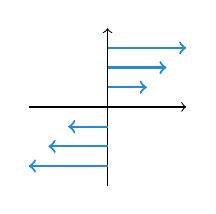
\begin{tikzpicture}[scale = 0.5]
      \draw[->] (-2,0) -- (2,0);
      \draw[->] (0,-2) -- (0,2);

      \draw[->, custom_blue, thick] (0,0.5) -- (1,0.5);
      \draw[->, custom_blue, thick] (0,1) -- (1.5,1);
      \draw[->, custom_blue, thick] (0,1.5) -- (2,1.5);

      \draw[->, custom_blue, thick] (0,-0.5) -- (-1,-0.5);
      \draw[->, custom_blue, thick] (0,-1) -- (-1.5,-1);
      \draw[->, custom_blue, thick] (0,-1.5) -- (-2,-1.5);
    \end{tikzpicture}
  \end{center}
\end{minipage} \\[2ex]
The linear transformation $T$ described by $B$ send $(x,y) \in \mathbb{R}^2$ to $(x+y, y)$. This is a \textbf{horizontal shear}: it shifts every point horizontally by its $y$-coordinate. \\[2ex]
For every point $v \in \mathbb{R}^2$, $T(v)$ is on the same horizontal line as $v$. It follows that $T(v)$ is a scalar multiply of $v$, only if $v$ lies on the $X$-axis; in this case, $T(v) = v$. \\[2ex]
The characteristic polynomial of $B$ (and $T$) is:
$$
  \det(xI_2 - B) = \det\begin{bmatrix}
    x-1 & -1  \\
    0   & x-1
  \end{bmatrix} = (x-1)^2 = (\lambda - 1)^2 = 0
$$
The only eigenvalue is $\lambda = 1$, and it has \textbf{algebraic multiplicity} $2$, meaning it appears twice as a root of the characteristic polynomial. \\[2ex]
Its \textbf{geometric multiplicity} is only $1$, meaning its corresponding eigenspace is only 1-dimensional - just the line $y = 1$.

\subsection{Eigenvector for distinct eigenvalues are independent}
\begin{theorembox}{}{}
  Let $A \in M_n{\mathbb{R}}$ and $v_1, \ldots, v_k$ be eigenvector of $A$ in $\mathbb{R}^n$ corresponding to distinct eigenvalues $\lambda_1, \ldots, \lambda_k$ of $A$. \\[2ex]
  Then $\{v_1, \ldots, v_k\}$ is a linearly independent subset of $\mathbb{R}^n$.
\end{theorembox}
\noindent\textbf{Proof (for $k = 3$):}
Note that no two $v_1, v_2, v_3$ are multiples of each other, since they correspond to distinct eigenvalues. \\[2ex]
Suppose: $a_1v_1 + a_2v_2 + a_3v_3 = 0$ for some $a_i \in \mathbb{R}$. We want to show that $a_1 = a_2 = a_3 = 0$. \\
Multiplying on the left by $A$ gives:
$$
  a_1Av_1 + a_2Av_2 + a_3Av_3 = 0 \Longrightarrow a_1\lambda_1v_1 + a_2\lambda_2v_2 + a_3\lambda_3v_3 = 0
$$
and multiplying the same equation by $\lambda_1$ gives:
$$
  a_1 \lambda_1 v_1 + a_2 \lambda_1 v_2 + a_3 \lambda_1 v_3 = 0
$$
Subtract to get:
$$a_2(\lambda_1 - \lambda_2)v_2 + a_3(\lambda_1 - \lambda_3)v_3 = 0$$
Since $v_2$ and $v_3$ are linearly independent, and $lambda_1 - \lambda_2 \neq 0$ and $\lambda_1 - \lambda_3 \neq 0$, it follows that $a_2 = a_3 = 0$ and hence $a_1 = 0$.
\subsection{At most $n$ distinct eigenvalues}
The following consequence of the previous theorem shows that  a matrix can have at most $n$ distinct eigenvalues. We already knew this, since the eigenvalues are roots of a polynomial of degree $n$.
\begin{theorembox}{Corollary}{}
  Let $A \in M_N(\mathbb{R})$. Then $A$ has at most $n$ distinct eigenvalues in $\mathbb{R}$.
\end{theorembox}
\noindent\textbf{Proof:} \\
If $A$ has $k$ distinct eigenvalues, with corresponding eigenvectors $v_1, \ldots, v_k \in \mathbb{R}^n$, then $k$ cannot exceed the dimension of $\mathbb{R}^n$, since $\{v_1, \dots, v_k\}$ is a linearly independent set in $\mathbb{R}^n$.
\begin{theorembox}{Corollary}{}
  If $A \in M_n(\mathbb{R})$ has $n$ distinct eigenvalues, then $A$ is diagonalizable.
\end{theorembox}
\noindent\textbf{Proof:} \\
A set consisting of one eigenvector for each of the $n$ eigenvalues is linearly independent, so hence is a basis.

\subsection{Notes about determinants and characteristic polynomials}
\begin{enumerate}
  \item The \textbf{characteristic polynomial} of the square matrix $A \in M_n(\mathbb{R})$ is the determinant of $\lambda I_n - A$.
  \item If $t$ is a root of this polynomial, the $t$-eigenspace of $A$ is the nullspace of the matrix $tI_n - A$.
  \item The determinant of a diagonal or upper triangular matrix is the product of the entries on its main diagonal.
  \item A square matrix is \textbf{block diagonal} if its non-zero entries are all contained in square blocks along its diagonal. The determinant of a block diagonal matrix is the product of the determinants of its diagonal blocks.
  \item Similar matrices have the same characteristic polynomial and the same eigenvalues and eigenspace dimensions, since they represent the same linear transformation.
\end{enumerate}

\subsection{Multiplicity of Eigenvalues}
Suppose that $A$ and $B$ are similar square matrices, so that $B = P^{-1}AP$ for some invertible matrix $P$. Then
\begin{align*}
  \det(xI - B) & = \det(xI - P^{-1}AP)              \\
               & = \det(P^{-1}(xI)P - P^{-1}AP)     \\
               & = \det\left(P^{-1}(xI - A)P\right) \\
               & = \det P^{-1} \det(xI - A) \det P  \\
               & = \det(xI - A).
\end{align*}

If two matrices have the same characteristic polynomial, they are not necessarily similar. For example $\begin{bmatrix} 1 & 0 \\ 0 & 1 \end{bmatrix}$ and $\begin{bmatrix} 1 & 1 \\ 0 & 1 \end{bmatrix}$ have the same characteristic polynomial but are not similar.

\subsection{Multiplicity of Eigenvalues}
Let $\lambda$ be an eigenvalue of a matrix $A \in M_n(\mathbb{R})$. The \textbf{algebraic multiplicity} of $\lambda$ is the number of times that $\lambda$ occurs as a root of the characteristic polynomial. The \textbf{geometric multiplicity} is the dimension of the $t$-eigenspace of $A$.
\begin{examplebox}{}{}
  $$A = \begin{bmatrix}
      3 & 0 & 0 & 0 \\
      0 & 3 & 0 & 0 \\
      0 & 0 & 4 & 1 \\
      0 & 0 & 0 & 4
    \end{bmatrix}$$

  The matrix has two distinct eigenvalues, $3$ and $4$. Both have algebraic multiplicity $2$; the characteristic polynomial is $(\lambda - 3)^2(\lambda - 4)^2$.
  The 3-eigenspace has dimension 2, its elements are $\begin{bmatrix} a \\ b \\ 0 \\ 0 \end{bmatrix}$, for $a, b \in \mathbb{R}$.

  The 4-eigenspace only has dimension 1, its elements are $\begin{bmatrix} 0 \\ 0 \\ c \\ 0 \end{bmatrix}$, for $c \in \mathbb{R}$.

  This $A$ is not diagonalizable since it does not have four independent eigenvectors.
\end{examplebox}
\subsection{Geometric multiplicity $\leq$ Algebraic multiplicity}
\begin{theorembox}{}{}
  The geometric multiplicity of an eigenvalue is at most equal to its algebraic multiplicity.
\end{theorembox}
\noindent\textbf{Proof:} \\
Suppose that $t$ has geometric multiplicity $k$ as an eigenvalue of the square matrix $A \in M_n(\mathbb{R})$, and let $\{v_1, \dots, v_k\}$ be a basis for the $t$-eigenspace of $A$. \\[2ex]
Extend this to a basis $\mathcal{B}$ of $\mathbb{R}^n$, and let $P$ be the matrix whose columns are the elements of $\mathcal{B}$. Then the first $k$ columns of $P^{-1}AP$ have $t$ in the diagonal position and zeros elsewhere. \\[2ex]
It follows that $\lambda - t$ occurs at least $k$ times as a factor of $\det(\lambda I_n - P^{-1}AP)$, so the algebraic multiplicity of $t$ is at least $k$.
\begin{theorembox}{Corollary}{}
  A matrix is diagonalizable if and only if the geometric multiplicity of each of its eigenvalues is equal to the algebraic multiplicity
\end{theorembox}
\subsection{Key Takeaways}
\begin{takeaway-box}{}{}
\begin{itemize}
  \item The $B$ coordinates of a vector a linear transformation $T$ is given by:
        $$[T(v)]_B = P^{-1}AP[v]_B$$
  \item Two matrices are \textbf{similar} there exists an invertible matrix $P$ such that $B = P^{-1}AP$.
  \item \textbf{Eigenvector} a vector which when operated on by a given operator gives a scalar multiple of itself.
  \item \textbf{Eigenvalue} the scalar multiple of an eigenvector.
  \item \textbf{Characteristic polynomial} $\text{det}(\lambda I_n - A)$ is a polynomial in $\lambda$ whose roots are the eigenvalues of $A$.
  \item \textbf{Eigenspace} the set of all vectors $v$ such that $Av = \lambda v$ for a given eigenvalue $\lambda$.
  \item \textbf{Diagonalizability} a matrix is diagonalizable if it has a basis of eigenvectors.
  \item \textbf{Horizontal Shear} a shear mapping that shifts every point horizontally by its $y$-coordinate.
  \item \textbf{Algebraic multiplicity} the number of times an eigenvalue appears as a root of the characteristic polynomial.
  \item \textbf{Geometric multiplicity} the dimension of the eigenspace corresponding to an eigenvalue.
  \item The set of eigenvectors corresponding to distinct eigenvalues is linearly independent.
  \item Given a $n \times n$ matrix $A$, $A$ has at most $n$ distinct eigenvalues.
  \item If $A$ has $n$ distinct eigenvalues, then $A$ is diagonalizable.
  \item The geometric multiplicity of an eigenvalue is $\leq$ to its algebraic multiplicity.
  \item A matrix is diagonalizable if and only if the geometric multiplicity of each of its eigenvalues is equal to the algebraic multiplicity.
\end{itemize}
\end{takeaway-box}

\section{Inner Products, Orthogonality, and Projections}
\section*{Introduction}
\noindent In this section, we introduce the notion of an \textbf{inner product}, a tool that lets us measure angles, lengths, and distances within a vector space—much like the dot product does in $\mathbb{R}^n$. Once we have an inner product, we can talk about \textbf{orthogonality}, or perpendicular vectors, which lays the groundwork for a host of geometric insights and computational techniques. \\[2ex]

\noindent First, we generalize the usual dot product to an arbitrary vector space by defining a function $\langle x, y \rangle$ that must satisfy certain symmetry, linearity, and positivity conditions. This innately geometric perspective extends to the concepts of \textbf{length} (or norm), \textbf{distance}, and \textbf{angle} in any such space. Orthogonality—where two vectors satisfy $\langle x, y \rangle = 0$—then becomes the keystone for analyzing how vectors project and decompose relative to each other. \\[2ex]

\noindent We examine how to build an \textbf{orthogonal basis}, a set of mutually perpendicular vectors that simplifies calculations significantly. The \textbf{Gram–Schmidt process} provides a systematic way to convert any basis into one that is orthogonal. Orthogonal bases enable us to define the \textbf{orthogonal projection} of a vector onto a subspace, i.e., the nearest point in the subspace to a given vector. This projection is at the heart of geometric approximations—particularly the solution of certain systems that may not have exact solutions. \\[2ex]

\noindent Finally, we apply these ideas to the method of \textbf{least squares} for \textbf{overdetermined systems}, where there are more equations than unknowns. By projecting the system’s right-hand side vector onto the column space of the coefficient matrix, we find an approximate solution that minimizes the total error. This illustrates just how powerful inner-product-based tools can be in both pure geometry and practical problem-solving contexts in data analysis, engineering, and beyond.

\subsection{Inner Products}
In $\mathbb{R}^n$, the dot product of the vectors $x = \begin{bmatrix}x_1 \\ x_2 \end{bmatrix}$ and $y = \begin{bmatrix}y_1 \\ y_2 \end{bmatrix}$ is defined as:
$$
  x \cdot y = x_1y_1 + x_2y_2 = x^T = y^T = y\cdot x
$$
When can interpret the length ($||x||$) of $x$ as the length of the line segment from origin to $(x_1, x_2)$, which by the Pythagorean theorem is:
$$
  \sqrt{x_1^2 + x_2^2} = \sqrt{x \cdot x}
$$
Once we have a concept of length, we can define distance ($d(x,y)$) between two vectors $x,y$ as the length of the line segment from $x$ to $y$, which is:
$$
  d(x,y) = ||x - y||
$$
Similarly, from the Cosine Rule:
$$x\cdot y = ||x|| \cdot ||y|| \cdot \cos(\theta)$$
where $\theta$ is the angle between $x$ and $y$. \\
We say that $x$ and $y$ are \textbf{orthogonal} (or $x \perp y$) if $x \cdot y = 0$. \\[2ex]
So the scalar product encodes geometric information in $\mathbb{R}^2$, and also provides a way to define length, distance and orthogonality. The scalar product is an example of an \textbf{inner product}.
\subsection{Real Inner Products}
A \textbf{{Inner Product}} on a vector space $V$ is a function from $V \times V$ to $\mathbb{R}$ that assigns an element of $\mathbb{R}$ to every ordered pair of elements of $V$, and has the following properties.

\begin{enumerate}
  \item \textbf{Symmetry}: $\langle x, y \rangle = \langle y, x \rangle$ for all $x, y \in V$
  \item \textbf{Linearity in both slots (bilinearity)}: For all $x, y, z \in V$ and all $a, b \in \mathbb{R}$, we have
        $\langle ax + by, z \rangle = a\langle x, z \rangle + b\langle y, z \rangle$ and
        $\langle x, ay + bz \rangle = a\langle x, y \rangle + b\langle x, z \rangle$.
  \item \textbf{Non-negativity}: $\langle x, x \rangle \geq 0$ for all $x \in V$, and $\langle x, x \rangle = 0$ only if $x = 0_V$.
\end{enumerate}

The ordinary scalar product on $\mathbb{R}^n$ is the best known example of an inner product.
\subsubsection{Examples of Inner Products}
\begin{enumerate}
  \item The ordinary scalar product on $\mathbb{R}^n$.

  \item Let $C$ be the vector space of all continuous real-valued functions on the interval $[0, 1]$. The analogue of the ordinary scalar product on $C$ is the inner product given by
        $$
          \langle f, g \rangle = \int_0^1 f(x)g(x)\, dx, \quad \text{for } f, g \in C.
        $$

  \item On the space $M_{m \times n}(\mathbb{R})$, the \textbf{Frobenius inner product} or \textbf{trace inner product} is defined by
        $$
          \langle A, B \rangle = \text{trace}(A^T B).
        $$
        Note that $\text{trace}(A^T B)$ is the sum over all positions $(i,j)$ of the products $A_{ij}B_{ij}$. So this is closely related to the ordinary scalar product, if the matrices $A$ and $B$ were regarded as vectors with $mn$ entries over $\mathbb{R}$.
\end{enumerate}

It is possible for a single vector space to have many different inner products defined on it, and if there is any risk of ambiguity we need to specify which one we are considering.
\subsection{Length, Distance and Scaling in an Inner Product Space}
\begin{definitionbox}{}{}
  We define the \textbf{length} or \textbf{norm} of any vector $v$ by:
  $$
    ||v|| = \sqrt{\langle v, v \rangle}
  $$
\end{definitionbox}
\begin{definitionbox}{}{}
  We define the distance between two vectors, $u$ and $v$, by:
  $$
    d(u, v) = ||u - v||
  $$
\end{definitionbox}
\begin{conceptbox}{Scaling}{}
  Every vector, $v$, and scalar, $c$, satisfy:
  $$
    ||cv|| = |c| \cdot ||v||
  $$
  Since:
  $$
    ||cv|| = \sqrt{\langle cv, cv \rangle} = \sqrt{c^2\langle v, v \rangle} = |c| \cdot ||v||
  $$
  So we can adjust the norm of any element of $V$ while preserving its direction, by multiplying by a scalar.
\end{conceptbox}
\begin{definitionbox}{}{}
  If $v$ is a non-zero vector in an inner product space $V$, then
  $$
    \hat{v} := \frac{1}{\|v\|}v
  $$
  is a unit vector in the direction of $v$, called the \textbf{normalization} of $v$.
\end{definitionbox}
\subsection{Orthogonality in an inner product space}
Let $V$ be a vector space with an inner product $\langle \cdot, \cdot \rangle$ (such as the ordinary scalar product).
\begin{definitionbox}{}{}
  We say that the vectors $u$ and $v$ are \textbf{orthogonal} (with respect to $\langle \cdot, \cdot \rangle$) if $\langle u, v \rangle = 0$.
\end{definitionbox}

All these definitions are consistent with “typical” geometrically motivated concepts of distance and orthogonality.
\textbf{Examples}
\begin{enumerate}
  \item $(2, 5)$ and $(5, -2)$ are orthogonal with respect to the ordinary scalar product in $\mathbb{R}^2$.

  \item $\sin \pi x$ and $\cos \pi x$ are orthogonal with respect to the scalar product on the space of continuous functions on $[0, 1]$ defined in Lecture 18; this is saying that
        $$
          \int_0^1 \sin(\pi x) \cos(\pi x) \, dx = 0 \quad \left(= \left. \frac{1}{2\pi} \sin^2(\pi x) \right|_0^1 \right).
        $$
\end{enumerate}
\subsection{Orthogonal Projection}
\begin{lemmabox}{}{}
  Let $u$ and $v$ be non-zero vectors in an inner product space $V$.
  Then it is possible to write (in a unique way) $v = au + v'$, where $a$ is a scalar and $v'$ is orthogonal to $u$.
\end{lemmabox}

\begin{itemize}
  \item If $v$ is orthogonal to $u$, take $a = 0$ and $v' = v$.

  \item If $v$ is a scalar multiple of $u$, take $au = v$ and $v' = 0$.

  \item Otherwise, to solve for $a$ and $v'$ in the equation $v = au + v'$ (with $u \perp v'$), take the inner product with $u$ on both sides. Then
        $$
          \langle u, v \rangle = a \langle u, u \rangle + 0 \Longrightarrow a = \frac{\langle u, v \rangle}{\|u\|^2}, \quad
          v' = v - \frac{\langle u, v \rangle}{\|u\|^2} u.
        $$
\end{itemize}
We can verify directly that the two components in this expression are orthogonal to each other. \\[2ex]
\noindent \textbf{Example}
$$\text{Write } u = \begin{bmatrix} 2 \\ 1 \end{bmatrix},\quad v = \begin{bmatrix} 6 \\ -2 \end{bmatrix} \quad \text{Then } u = \begin{bmatrix} \frac{3}{2} \\ \frac{3}{4} \end{bmatrix} + \begin{bmatrix} \frac{3}{2} \\ -\frac{11}{4} \end{bmatrix}$$

\subsection{Orthogonal projection of one vector on another}
\begin{definitionbox}{}{}
  For non-zero vectors $u$ and $v$ in an inner product space $V$, the vector
  $$
    \frac{\langle u, v \rangle}{\|u\|^2} u
  $$
  is called the projection of $v$ on the 1-dimensional space spanned by $u$. \\
  It is denoted by $\text{proj}_u(v)$ and it has the property that $v - \text{proj}_u(v)$ is orthogonal to $u$
\end{definitionbox}
\begin{lemmabox}{}{}
  $\text{proj}_u(v)$ is the unique element of $\langle u \rangle$ whose distance from $v$ is minimal.
\end{lemmabox}
\noindent \textbf{Proof:} Let $au$ be a scalar multiple of $u$. Then
$$
  d(au, v)^2 = \langle au - v, au - v \rangle = a^2 \langle u, u \rangle - 2a \langle u, v \rangle + \langle v, v \rangle
$$
Regarded as a quadratic function of $a$, this has a minimum when its derivative is 0, i.e. when
$$
  2a \langle u, u \rangle - 2 \langle u, v \rangle = 0, \quad \text{when } a = \frac{\langle u, v \rangle}{\|u\|^2}.
$$
\subsection{Orthogonal Bases (the Gram-Schmidt process)}
\begin{conceptbox}{}{}
  Every finite-dimensional inner product space has an \textbf{orthogonal basis}
\end{conceptbox}
\noindent We can start with any basis $\{b_1, \dots, b_n\}$, and adjust the elements one by one (by subtracting off orthogonal projections of later vectors on earlier ones). The process ends with an orthogonal basis $\{v_1, \dots, v_n\}$.

\begin{enumerate}
  \item Set $v_1 = b_1$, and
        \[
          v_2 = b_2 - \text{proj}_{v_1}(b_2) = b_2 - \frac{\langle v_1, b_2 \rangle}{\langle v_1, v_1 \rangle} v_1.
        \]
        Then the pairs $b_1, b_2$ and $v_1, v_2$ span the same space, and $v_1 \perp v_2$.

  \item Write $v_3 = b_3 - \text{proj}_{v_1}(b_3) - \text{proj}_{v_2}(b_3)$.
        Then $\{v_1, v_2, v_3\}$ and $\{b_1, b_2, b_3\}$ span the same space, and $v_3 \perp v_1$, $v_3 \perp v_2$. To see this look at $\langle v_3, v_1 \rangle$ and $\langle v_3, v_2 \rangle$, noting that
        \[
          v_3 = b_3 - \frac{\langle b_3, v_1 \rangle}{\langle v_1, v_1 \rangle} v_1 - \frac{\langle b_3, v_2 \rangle}{\langle v_2, v_2 \rangle} v_2.
        \]

  \item Continue: at the $k$th step, form $v_k$ by subtracting from $b_k$ its projections on $v_1, \dots, v_{k-1}$.
\end{enumerate}
\subsection{Orthogonal projection on a subspace}
The result of this process is a basis $\{v_1, \dots, v_n\}$ whose elements satisfy
$$
  \langle v_i, v_j \rangle = 0 \text{ for } i \ne j
$$
We can adjust this basis to a \textbf{orthonormal basis} (consisting of orthogonal unit vectors) by replacing each $v_i$ with its normalization $\hat{v}_i$.
From the Gram–Schmidt process, we have

\begin{theorembox}{}{}
  If $V$ is a finite-dimensional inner product space, then $V$ has an orthogonal (or orthonormal) basis.
\end{theorembox}
Now let $W$ be a subspace of $V$, and let $v \in V$. The \textbf{orthogonal projection} of $v$ on $W$, denoted $\text{proj}_W(v)$, is defined to be the unique element $u$ of $W$ for which
$$
  v = u + v',
$$
and $v' \perp w$ for all $w \in W$.
\subsection{Calculating the projection on a subspace}
\begin{examplebox}
  In $\mathbb{R}^3$, find the unique point of the plane $W : x + 2y - z = 0$
  that is nearest to the point $v : (1, 2, 2)$.
  \\ \rule{\textwidth}{1pt}\\
  First find an orthogonal basis for $W$: for example $\{b_1, b_2\}$, where
  $$
    b_1 = \begin{bmatrix} 1 \\ 0 \\ 1 \end{bmatrix}, \quad
    b_2 = \begin{bmatrix} 1 \\ -1 \\ -1 \end{bmatrix}
  $$

  Then
  \begin{align*}
    \text{proj}_W(v) & = \text{proj}_{b_1}(v) + \text{proj}_{b_2}(v)                                                                               \\
                     & = \frac{\langle b_1, v \rangle}{\langle b_1, b_1 \rangle} b_1 + \frac{\langle b_2, v \rangle}{\langle b_2, b_2 \rangle} b_2 \\
                     & = \frac{3}{2} b_1 - \frac{3}{3} b_2                                                                                         \\
                     & = \left( \frac{3}{2}, 0, \frac{3}{2} \right) - (1, -1, -1) = \left( \frac{1}{2}, 1, \frac{5}{2} \right)
  \end{align*}
\end{examplebox}
\subsection{$\text{proj}_{(v)}$ is the nearest point of W to v}
Let $u = \text{proj}_W(v)$ and let $w$ be any element of $W$.
Note that $v - u$ is orthogonal to both $w$ and $u$, hence to $w - u$. Then
\begin{align*}
  d(v, w)^2 & = \langle v - w, v - w \rangle                                                                 \\
            & = \langle (v - u) + (u - w), (v - u) + (u - w) \rangle                                         \\
            & = \langle v - u, v - u \rangle + 2 \langle v - u, u - w \rangle + \langle u - w, u - w \rangle \\
            & = \langle v - u, v - u \rangle + \langle u - w, u - w \rangle                                  \\
            & \geq d(v, u)^2,
\end{align*}
with equality only if $w = u = \text{proj}_W(v)$.
\subsection{Recall}
Let $u$ and $v$ be elements in an inner product space $V$. The \textbf{projection of $v$ on $u$} is
$$
  \text{proj}_u\,v = \frac{\langle u, v \rangle}{\langle u, u \rangle} u
$$
Then $\text{proj}_u\,v$ is the unique nearest element to $v$ of the 1-dimensional subspace spanned by $u$ (in the distance determined by the inner product), and
$$
  \langle v', u \rangle = 0,\quad v' \perp u,\quad \text{where } v' = v - \text{proj}_u\,v.
$$
So $v$ is the sum of its projection on $u$ and a component orthogonal to $u$. \\[2ex]
In general, if $W$ is any subspace of $V$ and $v \in V$, then there is a unique nearest element in $W$ to $v$, called $\text{proj}_W\,v$ or the \textbf{projection of $v$ on $W$},
and $v - \text{proj}_W\,v$ is orthogonal to \textbf{every element of $W$}.
\subsection{Orthogonal Basis}
An \textbf{orthogonal basis} of an inner product space $V$ is a basis whose elements are all orthogonal to each other.
\begin{theorembox}{}{}
  If $V$ is a finite-dimensional inner product space, then $V$ has an orthogonal (or orthonormal) basis.
\end{theorembox}
\noindent Let $\{v_1, \dots, v_n\}$ be any basis. We convert it to an orthogonal basis $\{b_1, \dots, b_n\}$ as follows.

\begin{enumerate}
  \item Set $b_1 = v_1$.
  \item Set $b_2 = v_2 - \text{proj}_{b_1} v_2$. Then $b_2 \perp b_1$ and
        $\text{span}(b_1, b_2) = \text{span}(v_1, v_2)$.
  \item Set $b_3 = v_3 - \text{proj}_{b_1} v_3 - \text{proj}_{b_2} v_3$.
        Then $b_3 \perp b_1$ and $b_3 \perp b_2$ and
        $\text{span}(b_1, b_2, b_3) = \text{span}(b_1, b_2, v_3) = \text{span}(v_1, v_2, v_3)$.
  \item Continue in this way: Set $b_k = v_k -$ (the sum of its projections on $b_1, \dots, b_{k-1}$).
\end{enumerate}

The result is an orthogonal basis of $V$.
\subsection{Projection on a subspace}
Let $W$ be a subspace of an inner product space $V$ and let $v$ be any element of $V$.\\
Then there is a unique element $w$ of $W$ for which
$v = w + v'$, and $v' \perp w$ for all $w \in W$. \\[2ex]
Then $w$ is called the \textbf{orthogonal projection of $v$ on $W$}, denoted $\text{proj}_W\,v$.
$$
  \text{proj}_W\,v = \text{proj}_{b_1}\,v + \cdots + \text{proj}_{b_k}\,v \quad \text{for an orthogonal basis } \{b_1, \dots, b_k\} \text{ of } W.
$$
\textbf{Example} \\
In $\mathbb{R}^3$, let $W$ be the subspace $x + y + 3z = 0$, and let $v = \begin{bmatrix} 1 \\ 1 \\ 1 \end{bmatrix}$.
Then
$$
  v = \begin{bmatrix} 1 \\ 1 \\ 1 \end{bmatrix}
  = \underbrace{\begin{bmatrix} 6/11 \\ 6/11 \\ -4/11 \end{bmatrix}}_{\text{proj}_W(v)}
  + \underbrace{\begin{bmatrix} 5/11 \\ 5/11 \\ 15/11 \end{bmatrix}}_{\perp W}
$$
\subsection{How to calculate $\text{proj}_W(v)$}
\begin{examplebox}{}{}
  In $\mathbb{R}^3$, let $W$ be the subspace $x + y + 3z = 0$, and let $v = \begin{bmatrix} 1 \\ 1 \\ 1 \end{bmatrix}$. Find an orthogonal basis of $W$
  \\ \rule{\textwidth}{1pt}\\
  For example $\{b_1, b_2\}$ with
  $$
    b_1 = \begin{bmatrix} -1 \\ 1 \\ 0 \end{bmatrix}, \quad
    b_2 = \begin{bmatrix} 3 \\ 3 \\ -2 \end{bmatrix}.
  $$

  Then
  \begin{align*}
    \text{proj}_W\,v & = \text{proj}_{b_1}\,v + \text{proj}_{b_2}\,v
    = \frac{\langle v, b_1 \rangle}{\langle b_1, b_1 \rangle} b_1 + \frac{\langle v, b_2 \rangle}{\langle b_2, b_2 \rangle} b_2 \\
                     & = \frac{0}{2} b_1 + \frac{4}{22} b_2 = \frac{4}{22} b_2
    = \begin{bmatrix} 6/11 \\ 6/11 \\ -4/11 \end{bmatrix}.
  \end{align*}

  $$
    v = \begin{bmatrix} 1 \\ 1 \\ 1 \end{bmatrix}
    = \underbrace{\begin{bmatrix} 6/11 \\ 6/11 \\ -4/11 \end{bmatrix}}_{\text{proj}_W(v)}
    + \underbrace{\begin{bmatrix} 5/11 \\ 5/11 \\ 15/11 \end{bmatrix}}_{\perp W}
  $$
\end{examplebox}
\begin{examplebox}
  In $\mathbb{R}^3$, find the unique point of the plane $W : x + 2y - z = 0$
  that is nearest to the point $v : (1, 2, 2)$.
  \\ \rule{\textwidth}{1pt}\\
  First find an orthogonal basis for $W$: for example $\{b_1, b_2\}$, where
  $$
    b_1 = (1, 0, 1), \quad b_2 = (1, -1, -1).
  $$
  Then
  \begin{align*}
    \text{proj}_W(v) & = \text{proj}_{b_1}(v) + \text{proj}_{b_2}(v)                                                                               \\
                     & = \frac{\langle b_1, v \rangle}{\langle b_1, b_1 \rangle} b_1 + \frac{\langle b_2, v \rangle}{\langle b_2, b_2 \rangle} b_2 \\
                     & = \frac{3}{2} b_1 - \frac{3}{3} b_2                                                                                         \\
                     & = \left( \frac{3}{2}, 0, \frac{3}{2} \right) - (1, -1, -1) = \left( \frac{1}{2}, 1, \frac{5}{2} \right).
  \end{align*}
\end{examplebox}
\subsection{Application: least squares for overdetermined systems}
\textbf{Example} Consider the following \textbf{overdetermined} linear system.
$$
  \begin{aligned}
    2x + y & = 3  \\
    x - y  & = 0  \\
    x - 3y & = -4
  \end{aligned}
  \quad \Longleftrightarrow \quad
  \begin{bmatrix}
    2 & 1  \\
    1 & -1 \\
    1 & -3
  \end{bmatrix}
  \begin{bmatrix}
    x \\
    y
  \end{bmatrix}
  =
  \begin{bmatrix}
    3 \\
    0 \\
    -4
  \end{bmatrix}
$$

This system has three equations and only two variables. It is inconsistent and \textbf{overdetermined} — each pair of equations has a simultaneous solution, but all three do not.

Overdetermined systems arise quite often in applications, from observed data.
Even if they do not have exact solutions, approximate solutions are of interest. \\[2ex]
For a vector $b \in \mathbb{R}^3$, the system
$$
  \underbrace{
    \begin{bmatrix}
      2 & 1  \\
      1 & -1 \\
      1 & -3
    \end{bmatrix}
  }_{A}
  \begin{bmatrix}
    x \\
    y
  \end{bmatrix}
  = b
$$
has a solution if and only if $b$ belongs to the 2-dimensional linear span $W$
of the columns of the coefficient matrix $A$:
$v_1 = \begin{bmatrix} 2 \\ 1 \\ 1 \end{bmatrix}$ and $v_2 = \begin{bmatrix} 1 \\ -1 \\ -3 \end{bmatrix}$.

If not, then the nearest element of $W$ to $b$ is $b' = \text{proj}_W(b)$, and our approximate solutions for $x$ and $y$ are the entries of the vector $c$ in $\mathbb{R}^2$
for which $Ac = b'$. We know that $b' - b$ is orthogonal to $v_1$ and $v_2$, which are the rows of $A^T$. Hence
$$
  A^T(b' - b) =
  \begin{bmatrix}
    0 \\
    0
  \end{bmatrix}
  \Longrightarrow A^T b' = A^T A c = A^T b \Longrightarrow
  c = (A^T A)^{-1} A^T b
$$
In our example,
$$
  \begin{bmatrix}
    2 & 1  \\
    1 & -1 \\
    1 & -3
  \end{bmatrix}
  \begin{bmatrix}
    x \\
    y
  \end{bmatrix}
  =
  \begin{bmatrix}
    3 \\
    0 \\
    -4
  \end{bmatrix}
$$

$$
  A = \begin{bmatrix} 2 & 1 \\ 1 & -1 \\ 1 & -3 \end{bmatrix}, \quad
  A^T = \begin{bmatrix} 2 & 1 & 1 \\ 1 & -1 & -3 \end{bmatrix}, \quad
  A^T A = \begin{bmatrix} 6 & -2 \\ -2 & 11 \end{bmatrix}, \quad
  A^T b = \begin{bmatrix} 2 \\ 15 \end{bmatrix}
$$
The least squares solution is given by
$$
  \begin{bmatrix}
    x \\
    y
  \end{bmatrix}
  = c = (A^T A)^{-1} A^T b =
  \frac{1}{62}
  \begin{bmatrix}
    11 & 2 \\
    2  & 6
  \end{bmatrix}
  \begin{bmatrix}
    2 \\
    15
  \end{bmatrix}
  =
  \begin{bmatrix}
    \frac{26}{31} \\
    \frac{47}{31}
  \end{bmatrix}
  .
$$

\end{document}
